\chapter{Fuzzy Set Theory}
This chapter draws upon foundational concepts and theoretical frameworks presented in \cite{FULLER1} and \cite{FULLER2}. 
% \section*{Motivation}
% Fuzzy sets were introduced by Zadeh in 1965 \cite{Zadeh1965}. 
% \signal{the example of tall people, we want to model imprecision and why probability theory is not well suited for this. También pensar si voy a diferenciar entre incertidumbre epistemológica o aleatoria, o si eso lo meto cuando hable de possibility.}

\section{Fuzzy Sets}
\signal{Decir cómo a partir de ese concepto de partial membership llegamos a esto y cómo es una generalización de boolean membership de classical sets. Di también que con classical y crisp nos referimos a boolean sets y con fuzzy a los otros. Di que usas la xi para la boolean membership y mu para la fuzzy en general}

\begin{definition}[Fuzzy Set]
    Let $X\neq\emptyset$ a set. Then we define a \textbf{fuzzy set A in X}, i.e., $A \in \fuzzy{X}$ as:
    \[A=\{(x,\mu_A(x))\mid x\in X\}\]
    Where $\mu_A:X\longrightarrow [0,1]$ is the \textbf{membership function} and $X$ is the \textbf{domain} of the fuzzy set.
\end{definition}

\begin{remark}
     Both the fuzzy set and the membership function uniquely identify each other.
\end{remark}

\begin{notation}{Notation}
    We may use \( A(x) \equiv \mu_A(x) \) interchangeably.
\end{notation}

\begin{definition}[Support]
    Let $A \in \fuzzy{X}$. The set of non zero membership value elements is called the support:
    \[\textnormal{Supp}(A)=\{x\in X \mid A(x)>0\}\]
\end{definition}

\signal{
\begin{definition}[Normal Fuzzy Set]
    A fuzzy set is called \textbf{normal} if there exists $x\in X$ such that $A(x)=1$. Otherwise it is called \textbf{subnormal}.
\end{definition}
}
\begin{definition}[$\alpha$-cut]
    Let $\alpha \in [0,1]$, the $\alpha$-cut (also called $\alpha$-cut) of a fuzzy set \( A \in \fuzzy{X}\) is:
    \[
    [A]^\alpha =
    \begin{cases}
    \{x \in X \mid A(x)\geq \alpha\} & \text{if } \alpha > 0, \\
    \textnormal{cl}(\textnormal{Supp}(A)) & \text{if } \alpha = 0.
    \end{cases}
    \]
    where \textit{cl} denotes the closure.
\end{definition}

\signal{
    \begin{definition}[Extremes of the support]
        
    \end{definition}
}


\begin{definition}[Fuzzy Subset]
    Given the fuzzy sets $A, B \in \fuzzy{X}$ we say $A$ is a fuzzy subset of $B$ (and write $A \subseteq B$) if and only if $A(x)
    \leq B(x) \forall x \in X$.

    Analogously, $A$ and $B$ are equal if and only if $A(x)=B(x) \forall x \in X$, i.e., each of them is a subset of the other.
\end{definition}

\begin{example}
    Here are some examples of common fuzzy sets:
    \begin{itemize}
        \item \textbf{Empty Fuzzy Set in $X$:} such that $\emptyset(x)=0 \forall x \in X$.
        \item \textbf{Universal Fuzzy Set in $X$:} such that $X(x)=1  \forall x \in X$.
        \item \textbf{Fuzzy Point in $X$:} such that $P(x_0)=1 \land A(x)=0 \forall x \in X-\{x_0\}$
        \item \textbf{Fuzzy Number:} Usually defined as a fuzzy set in $\mathbb{R}$ with some desirable properties. Will be covered in Section \ref{sec:fuzzy_numbers}.
    \end{itemize}
\end{example}

\section{Fuzzy Set Operations} \label{sec:set_operations}
% \begin{notation}[label={not:OpsFS}]{Notation for variables in the current section}
%     In this section, we use the variable \( x \) to represent time and \( y \) to represent distance.
%   \end{notation}

The notions of union and intersection in fuzzy sets were first introduced by Zadeh \cite{Zadeh1965} using the operations $\max\{A(x),B(x)\}$ and $\min\{A(x),B(x)\}$ respectively. These can be intuitively interpreted as follows: the union is the \textit{smallest} fuzzy set (having lowest membership values) that contains both sets, while the intersection is the \textit{biggest} fuzzy set (having highest membership values) that is contained by both sets.\\

However, these operations can be generalized by two broader classes of operators: triangular norms (for intersection) and triangular conorms (for union).

Triangular norms were first introduced by Karl Menger in 1942 \cite{OriginTNorms} in the context of probabilistic metric spaces. When generalizing distances between points to probability distributions (representing the probability that the distance is less than or equal to a given value), Menger defined an operation $T:\,[0,1]\times [0,1]\to [0,1]$ to preserve the triangular inequality. For points $x,y,z$ in a metric space with distance function $d(\cdot,\cdot)$, this operation satisfies:

\begin{equation}\label{eq:Ftriangle_inequality}
d(x, z) \leq d(x, y) + d(y, z) \quad \longrightarrow \quad F_{xz}(t + s) \geq T(F_{xy}(t), F_{yz}(s)) \quad \forall t,s \geq 0
\end{equation}

This inequality means that the probability of $d(x,z)$ being less than $t+s$ must be at least the t-norm of the probabilities that $d(x,y)<t$ and $d(y,z)<s$. Note the change from $\leq$ to $\geq$ in the inequality. This is consistent with \textit{larger} probabilities indicating \textit{smaller} distances are more likely.\\

Since this originated in the context of distances, the following properties were required for an operator to be a t-norm\footnote{Associativity and one identity were not originally proposed by Menger but were later added by Sklar and Schweizer \cite{Sklar1983} in their refinement of triangular norms}:

\begin{itemize}
  \item \textbf{Symmetry:} The order of combining probabilities shouldn't matter, just as intersection of sets is commutative. That is, combining probabilities for distances $(x,y)$ and $(y,z)$ should give the same result regardless of order.
  
  \item \textbf{Associativity:} When combining multiple probabilities (e.g., for paths through points $x,y,z,w$), the grouping shouldn't affect the result. This extends the triangular norm to be consistent with polygonal inequalities, similar to how nested intersections satisfy $(A \cap B) \cap C = A \cap (B \cap C)$.
  
  \item \textbf{Monotonicity:} If the probability $F_{xy}(t)$ increases, then the lower bound for $F_{xz}(t+s)$ given by $T(F_{xy}(t), F_{yz}(s))$ should not decrease. This is analogous to how adding elements in crisp sets (or increasing membership degrees in fuzzy sets) cannot reduce the intersection set.
  
  \item \textbf{One Identity:} If $F_{yz}(s) = 1$ (meaning $d(y,z) < s$ with certainty), then $F_{xz}(t+s)$ depends only on $F_{xy}(t)$. This is analogous to how intersecting with the universal set preserves the original set.
\end{itemize}


% \say{The name \textit{triangular norm} refers to the fact that in the framework of probabilistic metric spaces, t-norms and t-conorms are used to generalize triangle inequality of ordinary metric spaces.}\cite{NGAN2018}\\

Therefore, the concept of intersection (conjunction) of fuzzy sets is generally represented by a triangular norm (also called a t-norm).

\begin{definition}[Triangular Norm]
    A mapping $T:[0,1]\times [0,1] \longrightarrow [0,1]$ that satisfies:
    \begin{romanenum}
      \item \textbf{Symmetricity:} $T(x,y) = T(y,x) \quad \oldforall x,y \in [0,1]$
      \item \textbf{Associativity:} $T(x,T(y,z)) = T(T(x,y),z) \quad \oldforall x,y,z \in [0,1]$
      \item \textbf{Monotonicity:} $T(x,y) \leq T(x',y') \quad \textnormal{if }x\leq x' \textnormal{ and } y\leq y' \quad \oldforall x,y,x',y' \in [0,1]$
      \item \textbf{One Identity:} $T(x,1) = T(1,x) = x \quad \oldforall x \in [0,1]$
    \end{romanenum}
    is called a triangular norm or t-norm. Defines the \textbf{intersection} of two fuzzy sets $A$ and $B$ on $X$ by giving the membership function as $(A \cap B) (x) = T(A(x),B(x)) \forall x \in X$ 
\end{definition}

Its dual operator can also be obtained by a similar reasoning as before, but instead of considering the probability distribution of finding both points closer than a given distance, it considers the probability distribution ($G_{uv}(t) = 1 - F_{uv}(t)$) of finding them further apart than that distance. In this case, both inequalities are $\leq$ since larger probabilities indicate that greater distances are more likely.
\begin{equation}\label{eq:Gtriangle_inequality}
d(x, z) \leq d(x, y) + d(y, z) \quad \longrightarrow \quad G_{xz}(t + s) \leq S(G_{xy}(t), G_{yz}(s))
\end{equation}

The reasoning regarding the properties is entirely analogous to the previous case, with the only difference being that $F_{uv}(t) = 1 \Leftrightarrow  G_{uv}(t) = 0$, and here the identity element is zero (union with the empty set).



\begin{definition}[Triangular Conorm]
  A mapping $S:[0,1]\times [0,1] \longrightarrow [0,1]$ that satisfies:
  \begin{enumerate}[(i)]\setlength{\itemindent}{2em}
    \item \textbf{Symmetricity:} $S(x,y) = S(y,x) \quad \oldforall x,y \in [0,1]$
    \item \textbf{Associativity:} $S(x,S(y,z)) = S(S(x,y),z) \quad \oldforall x,y,z \in [0,1]$
    \item \textbf{Monotonicity:} $S(x,y) \leq S(x',y') \quad \textnormal{if }x\leq x' \textnormal{ and } y\leq y' \quad \oldforall x,y,x',y' \in [0,1]$
    \item \textbf{Zero Identity:} $S(x,0) = S(0,x) = x \quad \oldforall x \in [0,1]$
  \end{enumerate}
  is called a triangular conorm or t-conorm. Defines the \textbf{union} of two fuzzy sets $A$ and $B$ on $X$ by giving the membership function as $(A \cup  B) (x) = S(A(x),B(x)) \forall x \in X$ 
    
\end{definition}

Complement was defined by Zadeh \cite{Zadeh1965} as\footnote{This is not the only definition that satisfies the axioms of a complement and is compatible with the classical limit, but it is the simplest one and will be used in this text. Other alternatives and their axioms can be found in \cite{Sladoje2007}. In \cite{Klement2000}, this is called the standard negation $N_s$.}:

\begin{definition}[Complement]
  The complement of a fuzzy set $A\in \fuzzy{X}$ is another fuzzy set with membership function given by $\overline{A}(x) \coleq 1 - A(x) \forall x\in X$
\end{definition}

Notice that this definition of complement is consistent with the classical definition of complement but implies that an element might have \textbf{non-zero partial membership} to both a fuzzy set and its complement: Let $A$ be a fuzzy set on $X$ and $x \in X / A(x)\notin \{0,1\}$ then $\overline{ A}(x)= 1 - A(x) \notin \{0,1\}$.\\

One consequence of this fact is that the union of a fuzzy set and its complement is not the total set in general. Analogously, the intersection will not the empty set in general. Those two properties that hold in classical sets but might not be true in fuzzy sets, are often called the \textbf{laws of excluded middle and of non-contradiction}, respectively.\\

However, there are t-norms and t-conorms such as the ones named after \luka that do satisfy both laws\footnote{Indeed, all continuous t-norms in agreement with non-contradiction are isomorphic to \luka \cite[p.~7]{LukasiewiczNonContrad}.}. Another example is the drastic t-norm which also satisfies the law of non-contradiction, but not the law of excluded middle. See example \ref{ex:basic_tnorms} for their formal expressions. \signal{All of this, has implications for the derived logic that will be explained in section \ref{sec:fuzzy_logic}. }\\

Another important property that classical union and intersection satisfy is De Morgan's Laws. For an arbitrary pair of t-norm and t-conorm, these laws are not automatically satisfied. However, there are specific pairs that do fulfill them. To illustrate the relationship between t-norms and t-conorms that satisfy De Morgan's Laws, we can use our probabilistic metric space analogy. Reconsidering the probabilistic metrics $F,G$ introduced earlier and substituting $F = 1 - G$ into equation \ref{eq:Ftriangle_inequality}, we obtain:

\[ G_{xz}(t + s) \leq 1 - T(1 - G_{xy}(t), 1 - G_{yz}(s))\]

Comparing this with equation \ref{eq:Gtriangle_inequality}, we can derive a relationship between t-norms and t-conorms\footnote{The relation from proposition \ref{prop:rel_tnorm_tconorm} directly mirrors the classical set union definition via intersection and negation ($A\cup B \coleq \neg (\neg A \cap \neg B)$), which can be visualized with a Venn diagram. Therefore, it is natural that this condition is equivalent to the De Morgan's Laws.}, which is formalized in the following proposition:

\begin{proposition}[Relationship between t-norm and t-conorm]\label{prop:rel_tnorm_tconorm}
  Given a t-norm $T$, the t-conorm is $S(a,b)\coleq 1 - T(1-a, 1-b)$ if and only if the union and intersection defined by that pair satisfy the De Morgan's Laws.
\end{proposition}
\begin{remark}
  It is easy to see that the previous relation is equivalent to $T(a,b) = 1-S(1-a, 1-b)$ which can be obtained simply by substituting $a'=1-a$ and $b'=1-b$, i.e., working with the complementary fuzzy sets.
\end{remark}

\begin{proof}
  Let $x\in X$, $A$, $B$ be fuzzy sets over $X$ with $a \coleq A(x)$ and $b \coleq B(x)$\\

  $\quad \boxed{\text{not}(A \text{ or } B) = (\text{not } A) \text{ and } (\text{not } B)}$\\
  [0.5em]
  $\overline{ S(a,b)} = T(\overline{ a}, \overline{ b}) \iff 1 - S(a,b) = T(1-a, 1-b) \iff S(a,b) = 1 - T(1-a, 1-b)$\\

  $\quad \boxed{\text{not}(A \text{ and } B) = (\text{not } A) \text{ or } (\text{not } B)}$\\
  [0.5em]
  $\overline{ T(a,b)} = S(\overline{ a}, \overline{ b}) \iff 1 - T(a,b) = S(1-a, 1-b) \iff T(a,b) = 1 - S(1-a, 1-b)$

\end{proof}

\signal{Creo que además de esto de las leyes de de Morgan, también nos da que el modus ponen funciona si se cumple la propiedad esa. Además no sé si se llama residual property.}

\signal{
  Lo de Archimedean sirve para el teorema 1.8.1 de \cite{FULLER2}. Y tb con la law of large numbers con LR-fuzzy numbers.}

  \signal{Strict T-norms iff satisfy conditional cancellation}

  \signal{Tambien lo de que la T-norm e distributiva con max/sup sirve para justificar la definicion del producto cartesiano, así que esa propiedad la tendré que meter por aquí igual.}


The following algebraic properties will be needed when defining fuzzy logics and to classify continuous t-norms \cite[Def.~2.1 \& 2.13]{Klement2000}:

\begin{definition}[Nilpotent Element and Nilpotent T-norm]
Let $T$ be a t-norm. An element $a \in ]0,1[$ is a \emph{nilpotent element} of $T$ if there exists $n \in \mathbb{N}$ such that $a_T^{(n)} = 0$, where $a_T^{(n)} = T(a, a_T^{(n-1)})$ with $a_T^{(1)}=a$.

A t-norm is called nilpotent if and only if it is continuous and every $a\in ]0,1[$ is nilpotent.
\end{definition}

\begin{definition}[Strict T-norm]
  A t-norm is called strict if it is continuous and strictly monotone.
\end{definition}


\begin{definition}[Zero Divisor]
Let $T$ be a t-norm. An element $a \in ]0,1[$ is a \emph{zero divisor} of $T$ if there exists $b \in ]0,1[$ such that $T(a,b)=0$.
\end{definition}

\begin{definition}[Idempotent Element]
  Let $T$ be a t-norm. An element $a \in [0,1]$ is an \emph{idempotent element} of $T$ if $T(a,a)=a$. The elements $0$ and $1$ are always trivial idempotent elements.
  \end{definition}
  

\begin{definition}[Archimedean T-norm]
A t-norm $T$ is \emph{Archimedean} if for each $(x,y) \in ]0,1[^2$ there is an $n \in \mathbb{N}$ with $x_T^{(n)} < y$. \cite[Def.~2.9]{Klement2000}  

In particular, a \textit{continuous} t-norm $T$ is Archimedean if and only if $T(x,x) < x \forall x \in ]0,1[$, i.e. it doesn't have non-trivial idempotent elements. \cite[Thm.~2.12]{Klement2000}
\end{definition}


When a t-norm is continuous and Archimedean, there's a crucial relationship between its algebraic properties. It cannot be simultaneously strict and possess nilpotent elements (or zero divisors):

\begin{theorem}{Algebraic properties of continuous Archimedean T-norms \cite[Thm.~2.18]{Klement2000}}\label{thm:alg_arch_cont}
Let $T$ be a continuous Archimedean t-norm. Then the following are equivalent:
\begin{romanenum}
    \item $T$ is \emph{nilpotent}.
    \item There exists some nilpotent element of $T$.
    \item There exists some zero divisor of $T$.
    \item $T$ is not \emph{strict}.
\end{romanenum}
\end{theorem}

% \begin{remark}\label{rem:split_tnorms}
%   Continuous Archimedean t-norms can be splitted into two classes according to their nilpotent elements \cite[Cor.~3.30]{Klement2000}: strict (having no nilpotent elements except $0$) and nilpotent (where every element in $]0,1[$ is nilpotent).
% \end{remark}


  \begin{example}[Basic T-norms {\cite[Ex.~1.2]{Klement2000}}]\label{ex:basic_tnorms}
    These four t-norms are canonical examples because they represent the extremal and most representative cases with respect to the order relation (see definition \ref{def:weaker}) and algebraic properties. From weaker to stronger they are: $T_D \leq T_L \leq T_P \leq T_M$. 
    
    All of them are plotted in figures \ref{fig:2D_tnorms} and \ref{fig:tnorms_3D_plots}.
      \begin{itemize}
        \item \textbf{Minimum ($T_M$):} 
            This is the strongest t-norm (\cite[Rem.~1.5(i)]{Klement2000}). Every element is idempotent (indeed it is the only t-norm satisfying that \cite[Lem.~1.2.3]{FULLER2} \signal{igual este paréntesis debería escribirlo como un resultado mejor}), therefore it is not Archimedean. It has no zero divisors and no nilpotent elements other than 0.
    
        \[T_M(x, y) = \min(x, y) \quad S_M(x, y) = \max(x, y)
    \]
        \item \textbf{Product ($T_P$):} 
        This t-norm is strict Archimedean (\cite[Ex.~2.14(i)]{Klement2000}). It has only $0$ and $1$ as idempotent elements, no nilpotent elements (other than $0$), and no zero divisors (\cite[Ex.~2.2(i)]{Klement2000}).
        \[T_P(x, y) = x \cdot y \quad S_P(x, y) = x + y - x \cdot y\]
        \item \textbf{Łukasiewicz ($T_L$):} 
        This t-norm is nilpotent Archimedean (\cite[Ex.~2.14(i)]{Klement2000}). It has only $0$ and $1$ as idempotent elements. Every $a \in ]0,1[$ is a nilpotent element and also a zero divisor (\cite[Ex.~2.2(i)]{Klement2000}).
        \[T_L(x, y) = \max(0, x + y - 1) \quad S_L(x, y) = \min(1, x + y)\]
        \item \textbf{Drastic Product ($T_D$):} This is the weakest t-norm (\cite[Rem.~1.5(i)]{Klement2000}). It is Archimedean since $T_D(x,x)=0 < x$ for $x \in ]0,1[$. It has only $0$ and $1$ as idempotent elements. Every $a \in ]0,1[$ is a zero divisor, and also nilpotent (since $a_D^{(2)} = T_D(a, T_D(a,a)) = T_D(a,0) = 0$ for $a<1$). It is not continuous.
        \[T_D(x, y) = \begin{cases} \min(x,y) & \text{if } \max(x,y)=1 \\ 0 & \text{otherwise} \end{cases} \quad S_D(x, y) = \begin{cases} \max(x,y) & \text{if } \min(x,y)=0 \\ 1 & \text{otherwise} \end{cases}\]
      \end{itemize}
    \end{example}


\begin{figure}[ht]
    \centering
    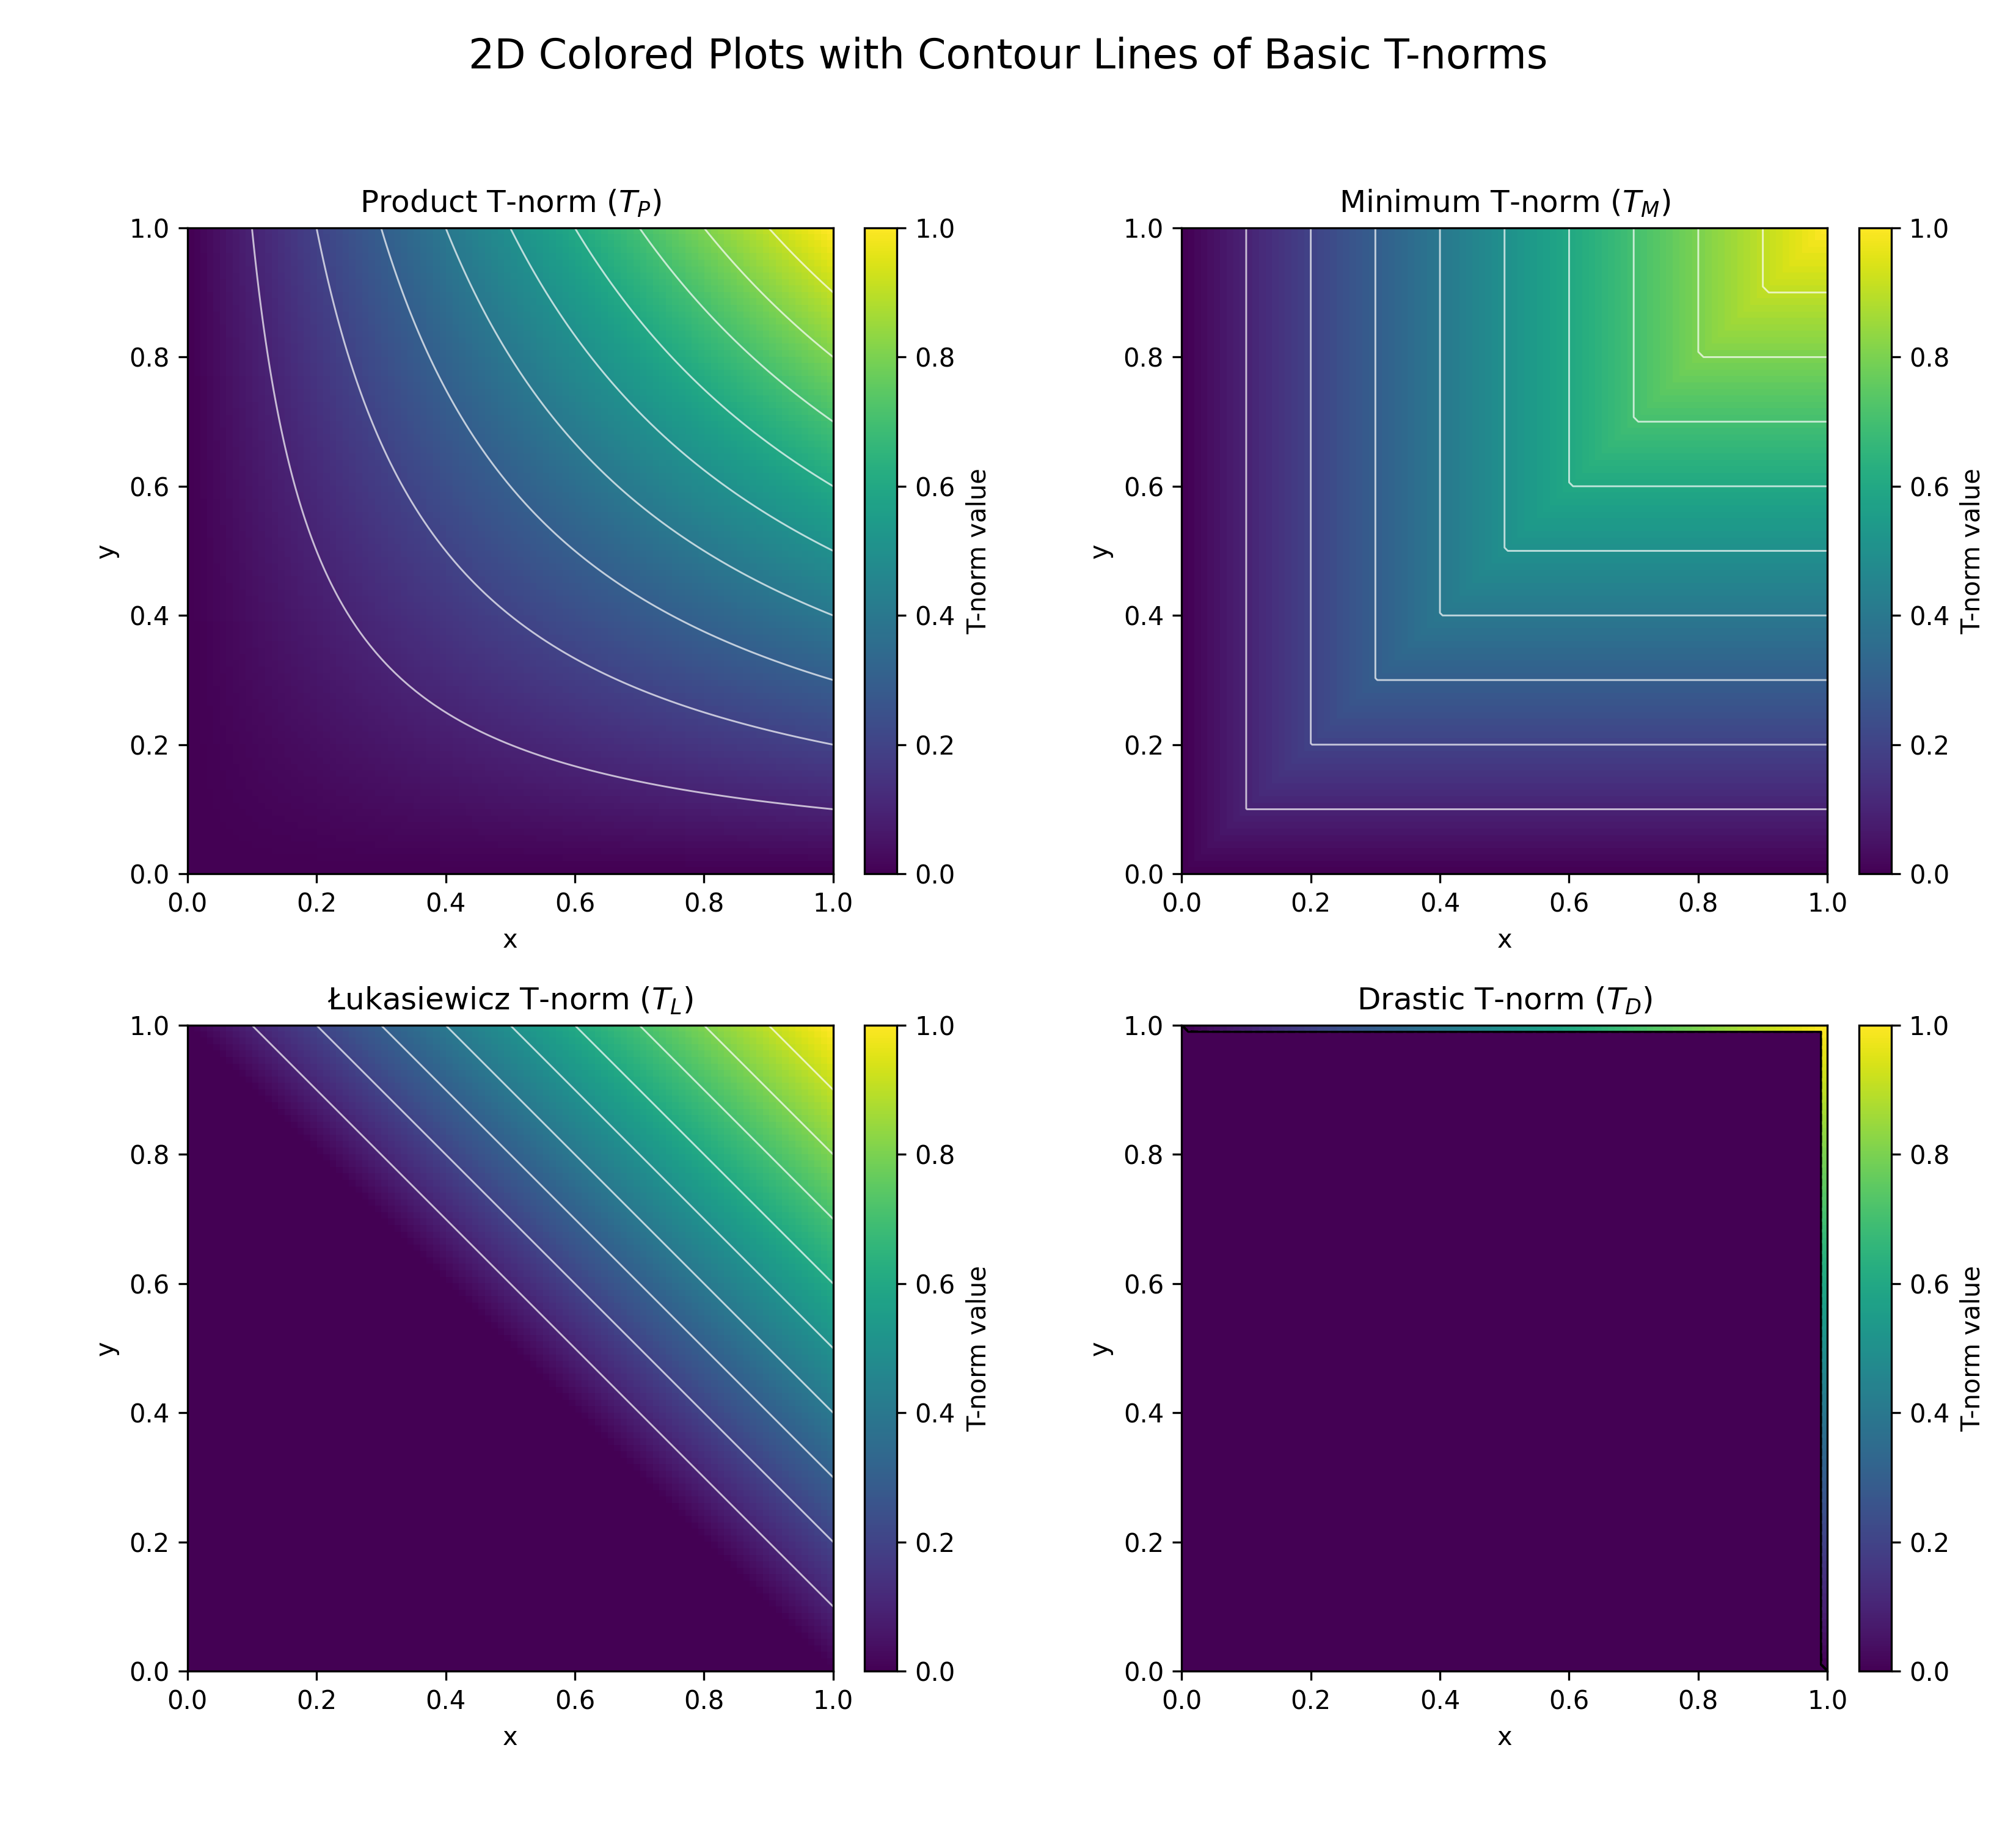
\includegraphics[width=0.85\textwidth]{ch1/figures/tnorms_2D_plots.png}
    \caption{Level curves of basic t-norms ($T_M$, $T_P$, $T_L$, $T_D$) in the unit square $[0,1]^2$. The different shapes of the white level curves illustrate the distinct behaviors and algebraic properties of each t-norm.}
    \label{fig:2D_tnorms}
\end{figure}


\begin{figure}[!ht]
    \centering
    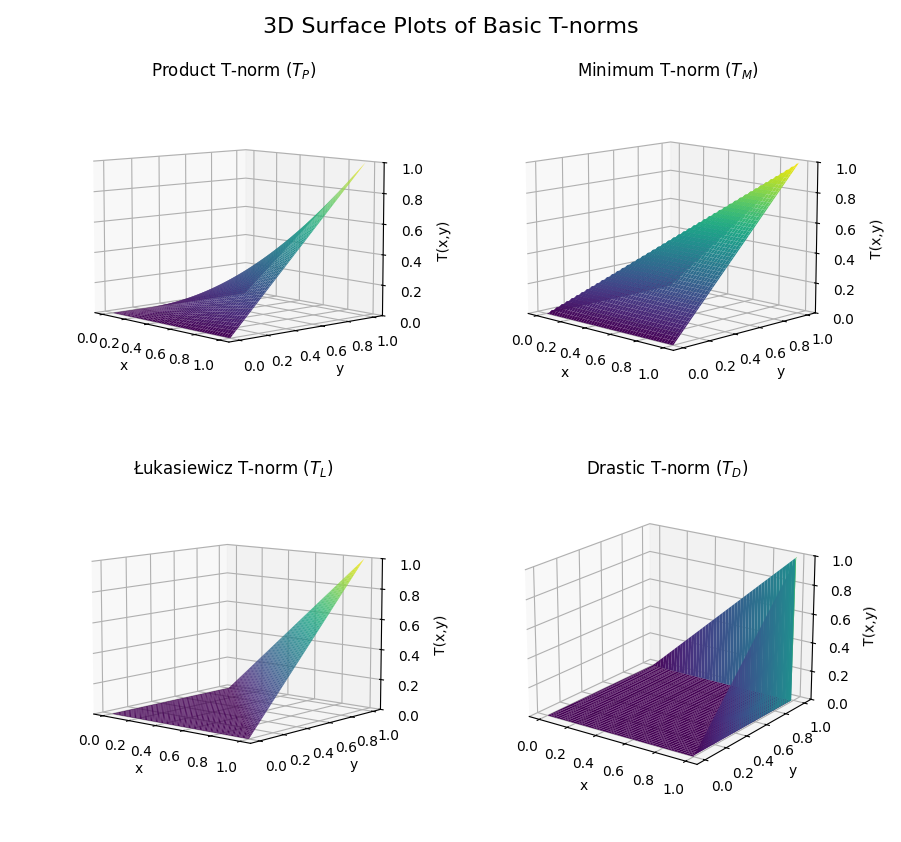
\includegraphics[width=0.95\textwidth]{ch1/figures/tnorms_3D_plots.png}
    \caption{3D surface plots of the basic t-norms ($T_M$, $T_P$, $T_L$, $T_D$) over the unit square $[0,1]^2$. The minimum t-norm forms a sharp ridge along $x=y$, the product t-norm is smoothly curved, the Łukasiewicz t-norm is planar except for a triangular region where it is zero, and the drastic t-norm is flat except for the edges. All of them are identical at the boundaries of the unit square.}
    \label{fig:tnorms_3D_plots}
\end{figure}


\subsection{Classification of T-norms}\label{sec:class_tnorms}
The first and most straight forward way to classify them is by defining the following partial order on the set of all t-norms. 
\begin{definition}[Weaker/Stronger t-norm {\cite[Def.~1.4]{Klement2000}}]\label{def:weaker}
  Given two t-norms $T_1$ and $T_2$, $T_1$ is said to be \emph{weaker} than $T_2$ (denoted $T_1 \leq T_2$) if $T_1(x,y) \leq T_2(x,y) \forall x,y \in [0,1]$.
  Equivalently, $T_2$ is said to be \emph{stronger} than $T_1$.
\end{definition}

\begin{remark}
  It's a fundamental result that for any t-norm $T$, we have $T_D \leq T \leq T_M$, where $T_D$ and $T_M$ are the drastic and the minimum t-norms respectively (\cite[Rem.~1.5]{Klement2000}).
\end{remark}

The interpretation is that a weaker t-norm can be seen as a stricter and more pessimistic intersection (conjunction in the fuzzy logic derived), returning lower membership values than a stronger one. Notice that it is not a total order: there are pairs of t-norms where none of them is weaker than the other. Some examples, such as the product $T_P$ and Yager $T_2^Y$ (see \ref{ex:families_tnorms} for the definition of the Yager family) t-norms, are shown in \cite[Fig.~6.1]{Klement2000}.\\


Another way to classify t-norms is based on their continuity properties. Continuous t-norms can be divided into two main classes (Fig.~\ref{fig:tnorm_classification}): Archimedean and non-Archimedean t-norms. The Archimedean t-norms can be further subdivided into strict and nilpotent t-norms (using the theorem \ref{thm:alg_arch_cont})\footnote{This classification is also characterized by the behavior of their generator functions at 0. For a more detailed discussion and definitions related to generators, see Appendix \ref{app:generators_tnorms}}:

\begin{itemize}
    \item $T$ is \textbf{strict} if it doesn't have any nilpotent elements except $0$. This means $T(x,y)>0$ whenever $x,y > 0$. (\cite[Cor.~3.30(i)]{Klement2000}).
    \item $T$ is \textbf{nilpotent} if every element in $]0,1[$ is nilpotent. This implies that for any $x,y \in ]0,1[$, there exists $n$ such that $T(x, \dots, x)$ ($n$ times) is $0$. (\cite[Cor.~3.30(ii)]{Klement2000}).
\end{itemize}


\begin{figure}[ht]
\centering
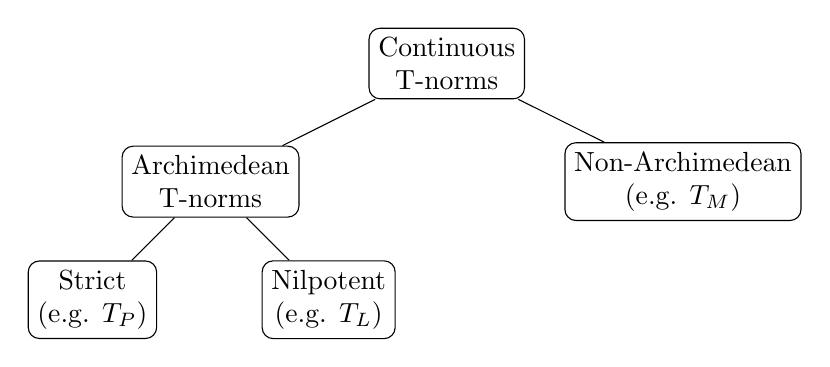
\begin{tikzpicture}[
    level 1/.style={sibling distance=60mm},
    level 2/.style={sibling distance=30mm},
    every node/.style={draw,rounded corners,align=center}
]
\node {Continuous\\ T-norms}
    child {
        node {Archimedean\\ T-norms}
        child {
            node {Strict\\ (e.g. $T_P$)}
        }
        child {
            node {Nilpotent\\ (e.g. $T_L$)}
        }
    }
    child {
        node {Non-Archimedean\\ (e.g. $T_M$)}
    };
\end{tikzpicture}
\caption{Classification of continuous t-norms}
\label{fig:tnorm_classification}
\end{figure}



Indeed, strict and nilpotent t-norms form two classes that are closed under certain isomorphic transformations: 

\begin{definition}[Isomorphic T-norms {\cite[Prop.~2.28(iv)]{Klement2000}}]
  Two t-norms $T_1$ and $T_2$ are \emph{isomorphic} if there exists a strictly increasing bijection $\varphi: [0,1] \to [0,1]$ (an automorphism of the unit interval) such that $T_2(x,y) = \varphi^{-1}(T_1(\varphi(x), \varphi(y)))$ for all $x,y \in [0,1]$.
\end{definition}
This definition is completely analogous for t-conorms. The isomorphism can be understood as a rescaling of the unit interval. The original t-norm is applied to this scaled domain and then the scale is reverted to make the output comparable to the original inputs $x,y$ (otherwise, the one identity property might not hold). Isomorphic t-norms share the same algebraic structure, merely operating on rescaled inputs and outputs via $\varphi$. A fundamental result is that (up to isomorphism) there are only two distinct types of continuous Archimedean t-norms: the product type and the Łukasiewicz type.
\begin{proposition}[{Classes of continuous Archimedean t-norms \cite[Cor.~5.7]{Klement2000}}]
  {\color{white}.}
  \begin{enumerate} 
      \item Every strict t-norm is isomorphic to the Product t-norm $T_P$.
      \item Every nilpotent t-norm is isomorphic to the Łukasiewicz t-norm $T_L$.
  \end{enumerate}
\end{proposition}

For general continuous t-norms that are not Archimedean, there must be non-trivial idempotent elements. These are constructed using ordinal sums.
\begin{definition}[Ordinal Sum of T-norms {\cite[Def.~3.44]{Klement2000}}]
Let $(T_\alpha)_{\alpha \in A}$ be a family of t-norms and $(]a_\alpha, e_\alpha[)_{\alpha \in A}$ be a family of non-empty, pairwise disjoint open subintervals of $[0,1]$. The t-norm $T$ defined by
\[
T(x,y) =
\begin{cases}
  a_\alpha + (e_\alpha - a_\alpha) \cdot T_\alpha \left( \frac{x-a_\alpha}{e_\alpha - a_\alpha}, \frac{y-a_\alpha}{e_\alpha - a_\alpha} \right) & \text{if } (x,y) \in [a_\alpha, e_\alpha]^2 \text{ for some } \alpha \in A \\
  \min(x,y) & \text{otherwise}
\end{cases}
\]
is called the \emph{ordinal sum} of the summands $(a_\alpha, e_\alpha, T_\alpha)$, $\alpha \in A$.
\end{definition}
Intuitively (see figure \ref{fig:ordinal_sum_tnorm}), an ordinal sum constructs a t-norm by combining scaled copies of other t-norms on the unit square $[0,1]^2$. For each interval $]a_\alpha, e_\alpha[$ along the main diagonal, a t-norm $T_\alpha$ operates within the square region $[a_\alpha, e_\alpha]^2$. Inside these "active" regions, inputs are first scaled down from $[a_\alpha, e_\alpha]$ to $[0,1]$ via linear transformations, then $T_\alpha$ is applied, and finally the result is scaled back to $[a_\alpha, e_\alpha]$. Outside these regions, the t-norm defaults to the minimum $T_M$, which ensures continuity (if the $T_\alpha$ are continuous) and makes the interval endpoints $a_\alpha, e_\alpha$ into idempotent elements of the resulting t-norm. This continuity at the boundaries of the active region is possible because any t-norm $T$ coincides with $T_M$ along the border of any square region centered in the diagonal $(x,x)$.\\

\begin{figure}[!ht]
    \centering
    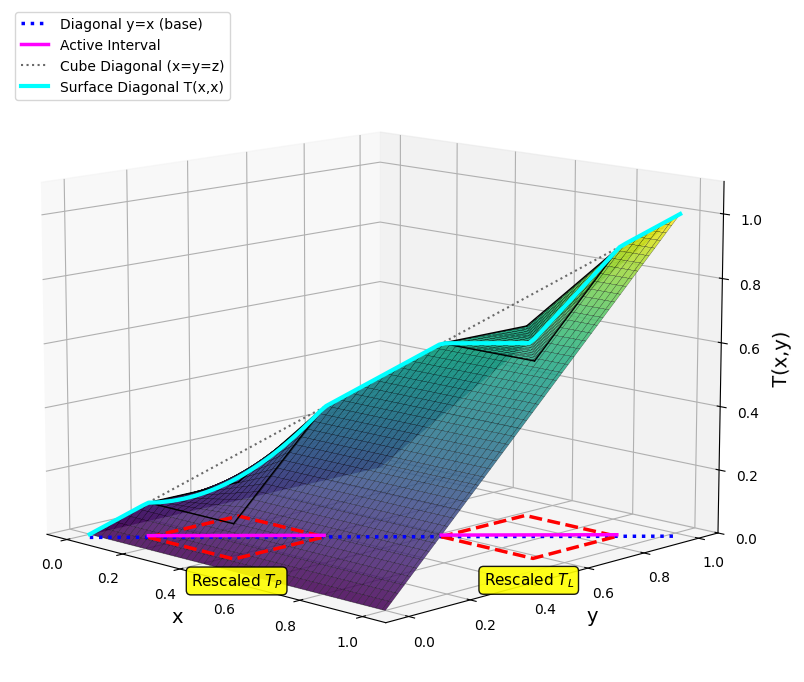
\includegraphics[width=0.9\textwidth]{ch1/figures/ordinal_sums.png}
    \caption{Visualization of an ordinal sum of t-norms. Each colored square (black on the surface, red on the xy plane) along the diagonal corresponds to an "active" region where a rescaled t-norm (Product or Łukasiewicz) operates. Outside these regions, the minimum t-norm $T_M$ is used. It is inspired by \cite[Fig.~3.16]{Klement2000}}
    \label{fig:ordinal_sum_tnorm}
\end{figure}



\begin{theorem}[Representation of Continuous T-norms {\cite[Thm.~5.11]{Klement2000}}]
  A function $T: [0,1]^2 \to [0,1]$ is a continuous t-norm if and only if $T$ is uniquely representable as an ordinal sum of continuous Archimedean t-norms.
\end{theorem}

The main idea behind this representation is leveraging the idempotent elements in the diagonal. Start with all the diagonal being idempotent (only possibility is $T_M$), and remove all the non-idempotent intervals (where the t-norm is locally Archimedean) with one of the two possibilities in the continuous case: strict (isomorphic to $T_P$) or nilpotent (isomorphic to $T_L$).

\begin{remark}
  If the family of subintervals is empty, the ordinal sum is defined as $T_M$.
\end{remark}

Unlike continuous t-norms, non-continuous t-norms generally lack a unifying framework based on generator functions that allows for a similar classification. Their analysis, therefore, focuses on the particular (semi-)continuity and algebraic characteristics. For examples and a discussion on semi-continuity of t-norms, see appendix \ref{app:cont_tnorms} and \ref{app:semicont-tnorms}.











































\section{Fuzzy Relations}
  In the previous sections we have been working with a single domain denoted by $X$. Intuitively, it might be useful to think about the domain as the different values of a property (independently of the object that has that property). For example, we could say that for the property \textit{lenght} the domain is $\R^+\coleq
  \{x\in\R \mid x \geq 0\}$ and a person might have a \textit{height} defined in that domain (modeled as a fuzzy set), although not all length values will be compatible with a person's height since it is safe to assume impossible to be 10 meters tall, but we do not know where to place a sharp boundary, so the feasible region of heights is best represented by a fuzzy set. If we were to look at the arm length, then we would have another set of feasible lenghts. Treating each set independently, doesn't allow to distinguish between the people of the same height with different arm lenght or viceversa. Therefore it is needed to a way to differentiate each unique combination of attributes. Notice that in this example, height and arm length have the same domain but for example hair color would have a different domain.\\

  Mathematically, this is done with relations which are subsets of the cartesian product of the domains, so that each element is a unique possible combination of attributes, an ordered n-tuple. For simplicity, let us consider just the cartesian product of 2 sets since the general case can be obtained inductively (see remark below). Again, the ``fuzzy" part will be referred to how we generalize the membership values to the continuum.


  \begin{definition}[Fuzzy Relation]
    Let $X\neq \emptyset \neq Y$ be classical sets. Then a fuzzy relation $R$ is a fuzzy set on $X\times Y$, i.e., $R\in \fuzzy{X\times Y}$. $R(x,y)$ will denote the degree of membership of $(x,y) \in R$.
  \end{definition}

  \begin{notation}[label={not:compositionFS}]{Notation}
    Although Fuzzy Relations are Fuzzy Sets as well, the name distinction will be used to denote whether the domain is a cartesian product or not.
  \end{notation}

  \begin{remark}
    To formally extend the Cartesian product from two sets to \( n \) sets using induction, it is important to observe that it satisfies associativity up to a natural isomorphism, i.e., 
    \[
    (A\times B)\times C \cong A\times (B\times C).
    \]
    and that t-norms satisfy the associativity property.
  \end{remark}

  Before giving the definition of the fuzzy cartesian product, we need to first understand what the classical cartesian product is in terms of the membership function. When we define a cartesian product $A\times B$ as "\textit{all unique ordered pairs of elements from $A$ \textbf{and} $B$}", in terms of membership functions we are taking the intersection of membership to $A$ and membership to $B$. Therefore, generalizing that notion with a t-norm we get the following definition.

  \begin{definition}[Fuzzy Cartesian Product]
    It is a fuzzy relation $A\times B \in \fuzzy{X\times Y}$ such that the membership function is given by:
    \[ 
    (A\times B)(x,y) = T(A(x), B(y)), \quad \forall (x,y) \in X\times Y
    \]
    where $T$ is a t-norm.
  \end{definition}

  To justify the definition of the membership function of a cartesian product of two fuzzy sets, let us first recall that in classical sets, we can retrieve the orginal subsets individually by taking the projection of the cartesian product. Given $R$ a relation on $X\times Y$ the projections are:

  \[\Pi_X(R)=\{x \in X \mid \exists y \in Y \textnormal{ such that } (x,y) \in R\}\]
  \[\Pi_Y(R)=\{y \in Y \mid \exists x \in X \textnormal{ such that } (x,y) \in R\}\]

  Then, with the boolean membership, it can be expressed as well as:

  \[\Pi_X(R)(x)=\sup\{R(x,y) \mid y\in Y\}=
  \begin{cases}
    1 & \textnormal{if } \exists y \in Y \textnormal{ such that } (x,y) \in R \\
    0 & \textnormal{otherwise}
  \end{cases}
  \]
  \[
    \Pi_Y(R)(y)=\sup\{R(x,y) \mid x\in X\}=
    \begin{cases}
      1 & \textnormal{if } \exists x \in X \textnormal{ such that } (x,y) \in R \\
      0 & \textnormal{otherwise}
    \end{cases}
  \]

  It is clear that in the case of having 2 possible values for the membership function, the above expresions are identical. The use of $\sup$ in the definition of the projection can be intuitively interpreted as the \textit{shadow} of the membership function of the cartesian product, as figure \ref{fig:class_cart_prod} illustrates. It is also desirable because then the following property holds for any classical cartesian product:\\
  $$ 
  \Pi_X(A\times B)=A \quad \textnormal{ and } \quad \Pi_Y(A\times B)=B \forall A\in X, \forall B \in Y
  $$

  \begin{figure}[ht]
    \centering
    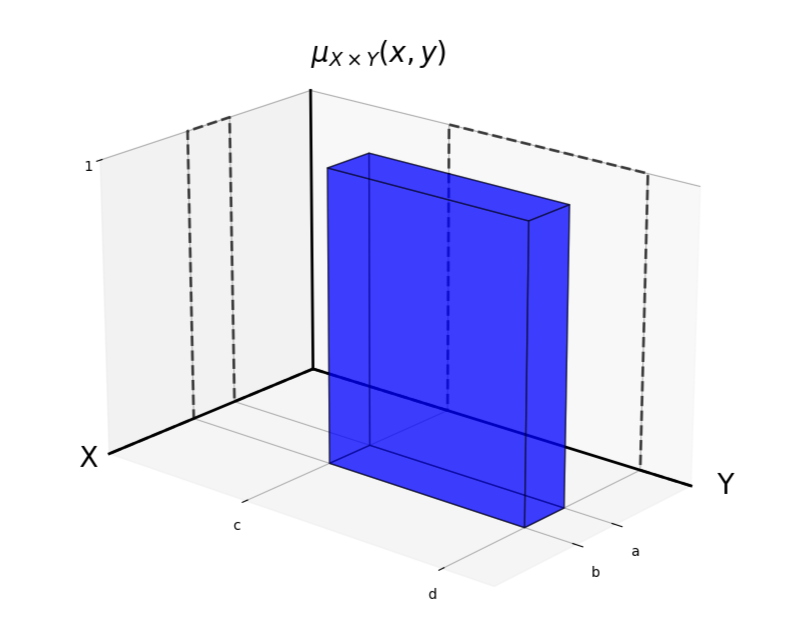
\includegraphics[width=0.65\textwidth]{ch1/figures/class_cart_prod.png}
    \caption{The blue volume represents the membership function of the cartesian product of two classical sets $X=[a,b]$ and $Y=[c,d]$ in $\R$. In the plane $y=0$ we have the projection that corresponds to the membership function of $X$ and analogously, the projection of $Y$ in the plane $x=0$.}
    \label{fig:class_cart_prod}
  \end{figure}

  Therefore, we define:

  \begin{definition}[Projection of a fuzzy relation]
    The projection from fuzzy relations on $X\times Y$ onto the fuzzy sets on $X$ is the function:
    \[
      \begin{aligned}
        \Pi_X: \fuzzy{X\times Y} &\longrightarrow \fuzzy{X} \\
        R &\longmapsto \Pi_X(R)
      \end{aligned}
    \]
    where $\Pi_X(R)(x) = \sup_{y\in Y}\{R(x,y)\}\forall x \in X$
  \end{definition}

  Applying the definition of projection with the supremum to fuzzy sets, we have a way to retrieve the membership function of each fuzzy set given the membership function of a fuzzy cartesian product (figure \ref{fig:fuzzy_cart_prod}). Therefore, any fuzzy cartesian product can be expressed as the fuzzy cartesian product of its own projections. This is justified in the following proposition: \\






  \begin{figure}[ht]
      \centering
      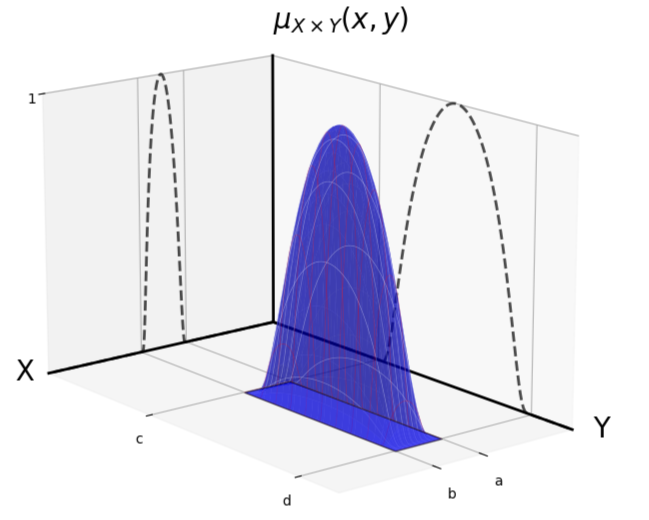
\includegraphics[width=0.65\textwidth]{ch1/figures/fuzzy_cart_prod.png}
      \caption{The blue volume represents the membership function of the cartesian product of two fuzzy sets $X$ and $Y$. In the plane $y=0$, we have the projection that corresponds to the membership function of $X$, and analogously, the projection of $Y$ in the plane $x=0$. The partial memberships illustrate how the fuzzy relations can vary across the domains.}
      \label{fig:fuzzy_cart_prod}
  \end{figure}



\begin{proposition}[Retrieval of Fuzzy Sets from their T-norm Cartesian Product]
  Let $A \in \fuzzy{X}$ and $B \in \fuzzy{Y}$ be fuzzy sets and $T$ a left-continuous t-norm. If the fuzzy set $B$ is normalized (i.e., $\sup\{B(y) \mid y \in Y\}  = 1$), then $\Pi_X(A \times B)(x) = A(x)$ for all $x \in X$. 
  In general, if $B$ is not normalized, we only get a lower bound $\Pi_X(A \times B)(x) \le A(x)$.
  \end{proposition}
  
  \begin{proof}
  \begin{equation*}
    \begin{split}
      \Pi_X(A \times B)(x) &= \sup_{y \in Y} T(A(x), B(y))= \\
      &= T(A(x), \sup_{y \in Y} B(y)) \leq
      \begin{cases}
        \min(A(x), 1) = A(x) & \text{if } B \text{ is normalized}\\
        \min(A(x), \sup_{y \in Y} B(y)) \leq A(x) & \text{otherwise}
      \end{cases}
    \end{split}
  \end{equation*}
  Since $A(x)$ is a constant with respect to the supremum over $y$, and t-norms are non-decreasing and left-continuous\footnote{If the function was only left-continuous but not non-decreasing, then that equality would instead be the $\geq$ inequality.} in their second argument, then the second equality holds. The inequality before the cases is justified using that the minimum t-norm is the strongest t-norm.
  \end{proof}
  
  \begin{remark}
  It is also crucial to emphasize that this retrieval is meaningful when the fuzzy relation $R$ under consideration is indeed a fuzzy Cartesian product of the form $A \times B$ using the t-norm $T$. If a given fuzzy relation $R'$ on $X \times Y$ is not $T$-decomposable (i.e., it cannot be expressed as $T(A'(x), B'(y))$ for any fuzzy sets $A'$ on $X$ and $B'$ on $Y$ with respect to the t-norm $T$), then the notion of retrieving original sets $A'$ and $B'$ from $R'$ doesn't make sense. While one can always compute the projections $A_P(x) = \Pi_X(R')(x)$ and $B_P(y) = \Pi_Y(R')(y)$, the relation $R'$ will not necessarily be equal to the $T$-Cartesian product of its projections, i.e., $R'(x,y) \neq T(A_P(x), B_P(y))$ in general for non-decomposable relations.
  \end{remark}


  Since infinitely many relations (including those that are not a fuzzy cartesian product) may have the same projections, it is not possible define the inverse operation. However, in the literature \cite[p.~61]{HistoryFL2017}, it is also defined the cylindric extension of a fuzzy set $A\in\fuzzy{X}$ as $CE_X(A)(x,y) = A(x)$. This operation is the simplest way to extend a fuzzy set to a relation ($\Pi_X(CE_X(A))=A$), and can be generalized to any n-ary relation as well.\\



\subsubsection*{Types of Fuzzy Relations on a Single Set}

When a binary fuzzy relation $R$ is defined on the Cartesian product of a single set with itself, it can characterize various ways in which elements of $X$ relate to themselves. Several properties, analogous to those in classical relations, are important for classifying these fuzzy relations \cite[p.~66]{HistoryFL2017}.

\begin{definition}[Properties of Binary Fuzzy Relations on $X^2$] Let $R \in \fuzzy{X \times X}$ (or $R \in \fuzzy{X^2}$) be a fuzzy binary relation, then:
  \begin{itemize}
    \item $R$ is \textbf{reflexive} if $R(x,x) = 1$ for all $x \in X$.
          Intuitively, every element is fully related to itself.
    \item $R$ is \textbf{symmetric} if $R(x,y) = R(y,x)$ for all $x,y \in X$.
          Intuitively, the degree of relationship from $x$ to $y$ is the same as from $y$ to $x$.
    \item $R$ is \textbf{transitive} (specifically, transitive under a t-norm $T$) if for all $x,y,z \in X$ and a given t-norm $T$,
          \[ T(R(x,y), R(y,z)) \le R(x,z). \]
          Using the definition of composition (see definition \ref{def:compos})this can be expressed as $R \supseteq R \circ R$. Often the minimum t-norm is used and it is then called sup-min transitive.
  \end{itemize}
\end{definition}

Based on these properties, two important types of fuzzy relations are:

\begin{definition}[Fuzzy equivalence relation]
  A fuzzy relation $S \in \fuzzy{X \times X}$ is A fuzzy equivalence relation (also called similarity relation) if it is reflexive, symmetric, and transitive (typically sup-min transitive).
\end{definition}
It generalizes the concept of a classical equivalence relation to the fuzzy context, indicating the degree to which elements are considered ``similar" or ``equivalent."

\begin{definition}[Fuzzy Compatibility Relation]
  A fuzzy relation $C \in \fuzzy{X \times X}$ is a \textbf{fuzzy compatibility relation} (also sometimes called a tolerance or proximity relation) if it is reflexive and symmetric.
\end{definition}
A fuzzy compatibility relation indicates that elements are compatible or close to each other, but this compatibility is not transitive. If $x$ is compatible with $y$, and $y$ with $z$, $x$ is not necessarily compatible with $z$ to the same degree.










\subsection{Composition of Fuzzy Sets}
\label{sec:compos}

The concept of projection allows us to combine fuzzy relations sharing a common domain. Intuitively, composing two fuzzy relations involves intersecting their membership values (using a t-norm) and then projecting the result onto the domain where the relations do not overlap.

\begin{definition}[Composition of Two Fuzzy Relations]\label{def:compos}
    Let \( R \in \fuzzy{X \times Y} \) and \( G \in \fuzzy{Y \times Z} \) be fuzzy relations sharing the set \(Y\). Their composition \( R \circ G \) is the fuzzy relation in \(\fuzzy{X \times Z}\) defined by
    \[
    (R \circ G)(x,z) = \Pi_{X\times Z}\Bigl[\, T\bigl(R(x,y), G(y,z)\bigr) \Bigr] = \sup_{y\in Y}\, T\bigl(R(x,y), G(y,z)\bigr),
    \]
    where \(T\) is a t-norm acting as the fuzzy intersection.
\end{definition}

% This means that given three properties $X$, $Y$ and $Z$ and two fuzzy relation R from X to Y and another fuzzy relation from Y to Z, we have a way to induce a relation $R\circ G$ between X and Z.

% (add a diagram here)

Given three sets \(X\), \(Y\), and \(Z\), suppose we have a fuzzy relation \(R\) from \(X\) to \(Y\) and another fuzzy relation \(G\) from \(Y\) to \(Z\). Using the composition operation, we can derive a new fuzzy relation \(R \circ G\) that directly connects \(X\) to \(Z\).

\noindent
\begin{minipage}{0.7\textwidth}
In this diagram, the arrows represent fuzzy relations, with \(R\) mapping elements from \(X\) to \(Y\), \(G\) mapping from \(Y\) to \(Z\), and \(R \circ G\) representing the induced fuzzy relation between \(X\) and \(Z\) through composition.\\
\end{minipage}%
\begin{minipage}{0.3\textwidth}
  \begin{center}
    \begin{tikzcd}
      X \arrow[r, "R", leftrightarrow] & Y \arrow[r, "G", leftrightarrow] & Z \arrow[bend right=30, from=1-1, "R \circ G"', leftrightarrow]
      \end{tikzcd}
  \end{center}

\end{minipage}


We can define a the composition of a fuzzy set with a fuzzy relation in a completely analogous way. 

\begin{definition}[Composition of a Fuzzy Set and a Fuzzy Relation]
    Let \( A \in \fuzzy{X} \) be a fuzzy set on \(X\) and \( R \in \fuzzy{X \times Y} \) be a fuzzy relation between \(X\) and \(Y\). The composition \( A \circ R \in \fuzzy{Y} \) is defined by
    \[
    (A \circ R)(y) = \Pi_{Y}\Bigl[\, T\bigl( A(x), R(x,y) \bigr) \Bigr] = \sup_{x \in X}\, T\bigl( A(x), R(x,y) \bigr),
    \]
    where \(T\) is a t-norm.
\end{definition}

\subsection{Extension Principle}

Following a similar idea as in the definition of the composition of fuzzy sets, we can derive a way to generalize crisp functions to fuzzy sets.\\

Let's consider the crisp function $f:\,X \longrightarrow Y$ where $X$ and $Y$ are classical sets. And consider as well the fuzzy sets $A \in \fuzzy{X}$. Then $f$ induces the classical relation $R=\{(x,y)\in X\times Y \mid f(x)=y\}$. And we can also make this relation fuzzy by copying the membership function of $A$:
$$ \mu_R (x,y) = \mu_A (x) \forall (x,y)\in R$$
Now we can define $B\in\fuzzy{Y}$, the fuzzy image of $A$ under $f$, as the projection of this fuzzy relation:
$$\mu_B (y) = \Pi_Y (R) = \sup\{R(x,y)\mid x\in X\} = \sup\{\mu_A (x)\mid x\in X, \, f(x)= y\} = \sup_{x\in f^{-1}(y)}\{\mu_A(x)\}$$

This is called the (Zadeh's) extension principle and is the basis for building arithmetic for fuzzy numbers (see section \ref{sec:fuzzy_numbers}) and generalizing any crisp function to fuzzy sets: 

\begin{definition}[Zadeh's extension principle]
  Let $f: X \longrightarrow Y$ be a crisp function and $A\in \fuzzy{X}$ a fuzzy set on $X$. Then we can define $f(A)\in \fuzzy{Y}$ as:
  \[
  \mu_{f(A)}(y)\equiv f(A)(y) = 
  \begin{cases}
    \sup_{x\in f^{-1}(y)}A(x) & \textnormal{if } f^{-1}(y)\neq \emptyset\\
    0 & \textnormal{otherwise}
  \end{cases}
  \quad\quad\quad \textnormal{where } f^{-1}(y)=\{x\in X \mid f(x)=y\}
  \]
\end{definition}


\begin{remark}
  If $f$ is \textbf{injective} then for any $y \in \textnormal{Im}(f)$ there exists a unique $x \in X$ such that $f(x)=y$, and therefore $f^{-1}(y)=\{x\}$. Then the first case can be rewritten as, $f(A)(y) = A(f^{-1}(y))$ if $y \in \textnormal{Im}(f)$.
\end{remark}

It is important to highlight as well that this definition is a straight forward generalization of set-valued functions where $f(A)= \{f(x)\mid x\in A\}$. In terms of boolean membership function:
$$\chi _{f(A)}(y)=\sup_{x\in f^{-1}(y)}\chi_A(x)$$

The definition above can be generalized to vector functions using the definition of fuzzy cartesian product, which requires us to take the intersection:

\begin{definition}[Sup-T extension principle]
  Let $f: X_1 \times \cdots \times X_n \longrightarrow Y$ be a crisp function and $A_1 \in \fuzzy{X_1}, \ldots, A_n \in \fuzzy{X_n}$ be fuzzy sets. Then we can define $f(A_1,\ldots,A_n)\in \fuzzy{Y}$ as:
  \[
  \mu_{f(A_1,\ldots,A_n)}(y)\equiv f(A_1,\ldots,A_n)(y) = 
  \begin{cases}
    \sup_{(x_1,\ldots,x_n)\in f^{-1}(y)} T(A_1(x_1),\ldots,A_n(x_n)) & \textnormal{if } f^{-1}(y)\neq \emptyset\\
    0 & \textnormal{otherwise}
  \end{cases}
  \]
  where $f^{-1}(y)=\{(x_1,\ldots,x_n)\in X_1\times\cdots\times X_n \mid f(x_1,\ldots,x_n)=y\}$ and $T$ is a t-norm.
\end{definition}

Which is again a generalization of vector set-valued functions where: $$f(A_1,\ldots,A_n)= \{f(x_1,\ldots,x_n)\mid x_i\in A_i\}$$
In terms of boolean membership function:
$$\chi _{f(A_1,\ldots,A_n)}(y)=\sup_{(x_1,\ldots,x_n)\in f^{-1}(y)}T(\chi_{A_1}(x_1),\ldots,\chi_{A_n}(x_n)) = \sup_{(x_1,\ldots,x_n)\in f^{-1}(y)}min\{\chi_{A_1}(x_1),\ldots,\chi_{A_n}(x_n)\}$$

Where we have used that every t-norm operates the same on boolean memberships.\\

\signal{Hay otros principios de extensión como el de Ramik con extensiones canónicas y order preserving operators, etc. No sé hasta qué punto eso podrá serme útil. Igual lo menciono en una frase y ya.}
\section{Fuzzy Numbers}\label{sec:fuzzy_numbers}
%See Nguyen paper page 7-8 of the pdf and 375-376 of the book.
According to Nguyen \signal{ (referenciar el paper de los teoremas de Nguyen)}:

\say{Interval analysis deals with closed bounded intervals (complex convex sets of $\R$) as an extension of numbers. Fuzzy numbers can be regarded as 
an extension of closed bounded intervals, [...]} 




\begin{definition}[Normal Fuzzy Set]
    A fuzzy set $A\in \fuzzy{X}$ is called \textbf{normal} if there exists $x\in X$ such that $A(x)=1$. Otherwise it is called \textbf{subnormal}.
\end{definition}

\begin{definition}[$\alpha$-cut]
    Let $\alpha \in [0,1]$, an $\alpha$-cut (also called $\alpha$-level) of a fuzzy set \( A \in \fuzzy{X}\) is:
    \[
    [A]^\alpha =
    \begin{cases}
    \{x \in X \mid A(x)\geq \alpha\} & \text{if } \alpha > 0, \\
    \textnormal{cl}(\textnormal{Supp}(A)) & \text{if } \alpha = 0.
    \end{cases}
    \]
    where \textit{cl} denotes the closure.
\end{definition}

\begin{remark}
    From the definition of $\alpha$-cut, the \textbf{nested property} states that for
    $\alpha_1, \alpha_2 \in ]0,1]$ if $\alpha_1\leq \alpha_2$ then $[A]^{\alpha_2}\subseteq [A]^{\alpha_1}$
\end{remark}

\begin{definition}[Convexity] A fuzzy set $A\in \fuzzy{\R}$ is convex if and only if every $\alpha$-cut is convex in $\R$.
    
\end{definition}

\begin{definition}[Fuzzy Number]
    A fuzzy number is a fuzzy set in the real line, i.e., $A\in \fuzzy{\R}$ such that:\vspace{-0.9em}
    \begin{romanenum}
        \item Normal\vspace{-0.5em}
        \item Convex\vspace{-0.5em}
        \item $\mu_A$ is continuous.\vspace{-0.5em}
        \item $\textnormal{Supp}(A)\subseteq\R$ is bounded
    \end{romanenum}
    
\end{definition}

\begin{proposition}[$\alpha$-cuts are closed intervals]
    Let $A\in \fuzzy{\R}$ be a fuzzy number. Then for every $\alpha \in [0,1]$, the $\alpha$-cut $[A]^\alpha$ is a closed interval in $\R$.
\end{proposition}

\begin{proof}
%1
The fact that $[A]^\alpha$ is an interval follows from the definition of convex subset in $\R$, which can only be an interval (or a single point).\\
%2
Now we prove that $[A]^\alpha$ is closed. For $\alpha \in (0,1]$, since $\mu_A$ is continuous and $[\alpha, 1]$ is closed in $\R$, the set
\[
[A]^\alpha = \mu_A^{-1}([\alpha, 1])
\]
is closed in $\R$. %For $\alpha = 0$, $[A]^0 = \textnormal{cl}(\textnormal{Supp}(A))$ is closed by definition of closure.
\end{proof}

\begin{notation}{Notation}
    We will denote the $\alpha$-cuts of a fuzzy number $A$ as 
    \[[A]^\alpha=[a_1(\alpha),a_2(\alpha)]\textnormal{ where }\begin{cases}
        a_1(\alpha)&=min[A]^\alpha\\
        a_2(\alpha)&=max[A]^\alpha\\
    \end{cases}\]
\end{notation}

\begin{note}
The condition of bounded support can be relaxed to define \textit{quasi-fuzzy numbers} \signal{(Which properties still hold and which are lost?)}:
$$\textnormal{(iv}_{\textnormal{bis}}\textnormal{) } \lim{t}{\infty}A(t) = 0 \quad \land \quad \lim{t}{-\infty}A(t) = 0$$
\end{note}

The following proposition establishes that the membership function of any fuzzy number can be partitioned into three contiguous intervals: one where it monotonically increases, one where it equals 1, and one where it monotonically decreases. This characterization shows that every fuzzy number can be represented as an LR-fuzzy number.

\signal{Esta proposición no me acuerdo de dónde la saqué.}

\signal{No sé si debería meterme en rollos de semicontinuidad inferior y superior de los extremos de los niveles.}

\begin{proposition}[Membership function of fuzzy numbers]
    Let $A\in \fuzzy{\R}$ be a fuzzy number, then it satisfies:
    \begin{romanenum}
        \item $\mu_A(t)=0$ outside an interval (denoted by $[a,d]$)\vspace{-0.5em}
        \item $\exists b,c \in \R \mid a\leq b \leq c \leq d$ where $\begin{cases}
            \mu_A\textnormal{ is monotone increasing in }[a,b]\\
            \mu_A\textnormal{ is monotone decreasing in }[b,d]\\
        \end{cases}$\vspace{-0.5em}
        \item $\mu_A(t)=1 \forall t\in [b,c]$
    \end{romanenum}
\end{proposition}


\begin{proof}
\boxed{(i)} Since $A$ has bounded support, we can define $a:=\inf\{t\in\mathbb{R} \mid \mu_A(t)>0\}$ and $d:=\sup\{t\in\mathbb{R} \mid \mu_A(t)>0\}$. Therefore $\mu_A(t)=0$ for all $t\notin[a,d]$. \\

\boxed{(iii)} Since $A$ is normal, we define $b:=\inf\{t\in\mathbb{R} \mid \mu_A(t)=1\}$ and $c:=\sup\{t\in\mathbb{R} \mid \mu_A(t)=1\}$. By continuity and convexity if there $\exists t\in [b,c]$ where $\mu_A(t)<1$, then $\exists \epsilon >0 \mid t\notin [A]^{t+\epsilon}$ is not a closed interval. Therefore we have $\mu_A(t)=1$ for all $t\in[b,c]$. \\

\boxed{(ii)} Since every $\alpha$-cut $[A]^\alpha=[a(\alpha),d(\alpha)]$ is a closed interval. The nested property of $\alpha$-cuts implies $a(\alpha)$ is non-decreasing and $d(\alpha)$ is non-increasing. For any $s,t\in[a,b]$ with $s<t$ and $\mu_A(s)=\alpha$, we have $t\in[A]^\alpha$, so $\mu_A(t)\geq\alpha=\mu_A(s)$. Similarly for $s,t\in[c,d]$ with $s<t$ and $\mu_A(t)=\alpha$, we have $s\in[A]^\alpha$, so $\mu_A(s)\geq\alpha=\mu_A(t)$. Therefore $\mu_A$ is monotone increasing on $[a,b]$ and monotone decreasing on $[c,d]$.
\end{proof}


% Write me a python function to represent the following fuzzy numbers in theree plots in the same figure. I want the letters to be the same as the ones in the definition and I want them all to be in the positive quadrant. Also write the 1 of the membership in the y axis saying that axis is the membership function of A \mu_A. The area of the fuzzy number must be gray and plot also thin lines for the reference values.
\begin{example}Here are some examples of fuzzy numbers:
    \begin{itemize}
        \item \textbf{Triangular Fuzzy Number:} Defined by a triplet $A\equiv(a, \alpha, \beta)$ where $a$ is the peak and $\alpha$ and $\beta$ the right and left widths respectively. The membership function $\mu_A(x)$ is given by:
        \[
        \mu_A(x) = 
        \begin{cases} 
        1-\frac{a-x}{\alpha} & \text{if } a \leq x < a-\alpha, \\
        1-\frac{x-a}{\beta} & \text{if } a+\beta < x \leq a, \\
        0, & \text{otherwise.}
        \end{cases}
        \]
        
        \item \textbf{Trapezoidal Fuzzy Number:} Defined by a quadruplet $A\equiv(a, b, \alpha, \beta)$ where $[a,b]$ is the tolerance interval and $\alpha$ and $\beta$ the right and left widths respectively. The membership function $\mu_A(x)$ is given by:
        \[
        \mu_A(x) = 
        \begin{cases} 
        1-\frac{a-x}{\alpha} & \text{if } a \leq x < a-\alpha, \\
        1, & \text{if } b \leq x \leq a, \\
        1-\frac{x-b}{\beta} & \text{if } b+\beta < x \leq b, \\
        0, & \text{otherwise.}
        \end{cases}
        \]
        
        \item \textbf{LR-Fuzzy Number:} Defined by a quadruplet $A\equiv(a, b, \alpha, \beta)$ where $[a,b]$ is the core (or peak) interval and $\alpha$ and $\beta$ the left and right widths respectively. The membership function $\mu_A(x)$ is given by:
        \[
        \mu_A(x) = 
        \begin{cases} 
        L\left(\frac{a-x}{\alpha}\right) & \text{if } a-\alpha \leq x < a, \\
        1, & \text{if } a \leq x \leq b, \\
        R\left(\frac{x-b}{\beta}\right) & \text{if } b < x \leq b+\beta, \\
        0, & \text{otherwise,}
        \end{cases}
        \]
        where $L$ and $R$ are continuous monotone non-increasing functions from $[0,1]$ to $[0,1]$ with $L(0)=R(0)=1$.
    \end{itemize}
\end{example}
    

\subsection{Nguyen's Theorems}
\signal{We use continuous functions because that way, we get the image of an interval is an interval as well. So then we get another fuzzy number because it maintains the convexity property?}

That is because the image under $f:\R \longrightarrow \R$ continuous of a compact is compact and of a connected set is a connected set. Therefore continuous functions move intervals to intervals.

\signal{This is for fuzzy numbers with the definition we gave them!}
%https://sci-hub.se/10.1016/0165-0114(91)90139-H
\begin{theorem}[First Nguyen Theorem]
    Let $f:\, \R \longrightarrow \R$ a continuous function and $A\in \R$ any fuzzy number \signal{(creo que vale para LR fuzzy num)}. Then,
    \[
    [f(A)]^{\alpha} = f([A]^{\alpha})=\{f(x)\mid x\in [A]^\alpha\}
    \]
    Moreover, if $f$ is monotonically increasing (if $f$ were decreasing, the order of the interval would be reversed), then:
    \[
    [f(A)]^{\alpha} = f([a_1(\alpha), a_2(\alpha)])=
    [f(a_1(\alpha)), f(a_2(\alpha))]
    \]
    where $[\cdot]^\alpha$ denotes the $\alpha$-cut of a fuzzy set and $a_1(\alpha), a_2(\alpha)$ the extremes of the $\alpha$-cut.
\end{theorem}

\signal{Sup- t-norm convolution para la generalización lo menciono?? Y eso de la convolución es útil para algo más?}

\begin{theorem}[Second Nguyen Theorem]
    Let $f:\, \R \times \R\longrightarrow \R$ a continuous function and $A,B$ \signal{any} fuzzy numbers. Then,
    \[
    [f(A,B)]^{\alpha} = f([A]^{\alpha},[B]^{\alpha})=\{f(x_1,x_2)\mid x_1\in [A]^\alpha, \, x_2\in [B]^\alpha\}
    \signal{=[A]^\alpha [B]^\alpha}
    \]
    where $[\cdot]^\alpha$ denotes the $\alpha$-cut of a fuzzy set.
\end{theorem}


\signal{generalization of Nguyen Theorems by Fuller in sectino 1.9 of Fuller 2.}



\subsection{Fuzzy Arithmetic}


\signal{
\subsection{Metrics for fuzzy numbers}}
\section{Fuzzy Measures: Probabilities and Possibilities.}
% \signal{Possibility is normalized so that 1 membership is attained at some point. And it models the compatibility of 2 states. That is of being 1.80 height and being tall states.

% Probability Models aleatoric uncertainty y Possibility models epistemic uncertainty?\\

% Probability-Possibility Transformations:
% Under certain conditions, one can associate a family of probability distributions with a given possibility distribution. For instance, the possibility distribution can be seen as an upper envelope for a set of probability measures that are consistent with the available imprecise information. Such transformations (e.g., the Dubois-Prade method) allow one to move between the two representations, albeit at the cost of introducing conservatism or ambiguity.\\


% Bayesian Models for modeling both uncertainties:\\

% Epistemic Uncertainty:

% Bayesian models explicitly account for uncertainty about the model parameters by placing a prior over them and computing a posterior after observing data. This kind of uncertainty reflects our lack of knowledge due to limited data and can be reduced by gathering more information.\\

% Aleatoric Uncertainty:

% This type of uncertainty represents the inherent noise in the data itself (for example, measurement error). In Bayesian modeling, aleatoric uncertainty is often incorporated into the likelihood function. It is considered irreducible since it stems from the randomness in the data generation process.\\

% Osea que a qué nos referimos con epistemologic uncertainty? A que nos falta info (data) o a que tenemos toda la info que se puede tener y no podemos reducir ese gap de incetidumbre porque es un problema de definición imprecisa. Tengo que diferenciar entre vagueza y epistemologico entonces?

% \subsection{Probability-Possibility Transformations}
% %https://www.researchgate.net/publication/2743789_On_PossibilityProbability_Transformations
% From the paper: \cite{Dubois1997}: 
% it is recalled in this paper that the probabilistic representations and the possibilisticones are not just two equivalent representations of uncertainty

% The possibilisticrepresentation is weaker because it explicitly handles imprecision (e.g. incompleteknowledge) and because possibility measures are based on an \textbf{ordering structure} rather than an \textbf{additive one}.

% the principle of insufficient reason from possibility toprobability, and the principle of maximum specificity from probability topossibility.

% Mencionar: consistency principle, principle of insufficient reason and principle of maximum specificity
% }






% \signal{Y HABLAR TAMBIÉN DE PLAUSIBILITY MEASURE Y CÓMO ESO SE RELACIONA CON EL LAS OTRAS MEASURES. MIRA EN Joseph Y. Halpern - Reasoning about Uncertainty-The MIT Press (2003)}


The study of fuzzy measures emerged as a generalization of classical measure theory, motivated by the increasing realization that the additivity axiom, fundamental in traditional measurement and probability theories as formalized by Borel, Lebesgue, and Kolmogorov, was often "too restrictive and, consequently, unrealistic" for modeling real-world complexities \cite[p.~10]{FuzzyMeasureHistory}. An alternative to classical measure theory came with Choquet's theory of capacities in 1954, followed by Dempster's and Shafer's development of belief and plausibility measures\footnote{Belief and plausibility measures are defined using a "basic probability assignment", which distributes a total measure of evidence across subsets $A_i \,(i\in \mathcal{I}\subseteq \N)$ of outcomes. When these subsets are "consonant" (they can be ordered with inclusion: $A_i \subseteq  A_{i+1}\forall i\in \mathcal{I}$), these measures become equivalent to possibility and necessity measures, respectively. This makes possibility and necessity special, highly structured cases within the broader Dempster-Shafer framework \cite[Thm.~3.23, Thm.~3.25]{FuzzyMeasureHistory}.} (superadditive and subadditive functions) in the late 1960s and 1970s to handle interval-valued probabilities. Simultaneously, the concept of a fuzzy set, introduced by Zadeh in 1965, laid the groundwork for possibility measures. It was within this context of fuzzy sets that Sugeno, in 1974, conceived fuzzy measures and fuzzy integrals, replacing the strict additivity requirement with weaker axioms of monotonicity and continuity, thereby paving the way for a more nuanced mathematical framework capable of capturing intrinsic nonadditive aspects of real-world phenomena like measurement errors and subjective judgments \cite[p.~13]{FuzzyMeasureHistory}.\\

\begin{definition}[Fuzzy Measure (Capacity)]
Let $\Omega$ be a universal set. A fuzzy measure (or capacity) $\nu$ is a set function
\[ \nu: 2^\Omega \to [0, 1] \]
that assigns a value to each subset of $\Omega$ (often called an event or criterion) such that:
\begin{enumerate}
    \item \textbf{Boundary Conditions:}
    \begin{itemize}
        \item $\nu(\emptyset) = 0$ (the measure of the empty set is zero).
        \item $\nu(\Omega) = 1$ (the measure of the universal set is one).
    \end{itemize}
    \item \textbf{Monotonicity:} For any $A, B \subseteq \Omega$, if $A \subseteq B$, then $\nu(A) \le \nu(B)$.
\end{enumerate}
\end{definition}

The crucial departure from classical probability (in its general form) is the absence of a strict additivity requirement for disjoint sets. This allows fuzzy measures to model situations where, for example, the combined importance of two criteria $A$ and $B$ might be greater than the sum of their individual importances (synergy) or less (redundancy). The value $\nu(A)$ quantifies the weight, importance, degree of belief, or capacity associated with the subset $A$.

A fuzzy measure $\nu$ is fundamentally defined by its $2^{|N|}$ values assigned to all subsets of the universal set $N$ \cite[p. 41]{beliakov2023discrete}. They are classified based on several criteria such as based on their behavior concerning additivity and modularity, which describe interactions between set contributions.
Regarding additivity, which considers disjoint sets $A,B \subseteq N$ (i.e., $A \cap B = \emptyset$):
\begin{itemize}
    \item a measure is additive if $\nu(A \cup B) = \nu(A) + \nu(B)$ \cite[Def. 2.4, Eq. 2.1]{beliakov2023discrete};
    \item it is subadditive if $\nu(A \cup B) \leq \nu(A) + \nu(B)$ \cite[Def. 2.10, Eq. 2.8]{beliakov2023discrete};
    \item and superadditive if $\nu(A \cup B) \geq \nu(A) + \nu(B)$ \cite[Def. 2.10, Eq. 2.9]{beliakov2023discrete}.
\end{itemize}
Modularity describes how the measure of unions and intersections relates to the sum of individual measures for any sets $A,B \subseteq N$:
\begin{itemize}
    \item a measure is submodular if $\nu(A \cup B) + \nu(A \cap B) \leq \nu(A) + \nu(B)$ \cite[Def. 2.8, Eq. 2.3]{beliakov2023discrete};
    \item it is supermodular if $\nu(A \cup B) + \nu(A \cap B) \geq \nu(A) + \nu(B)$ \cite[Def. 2.8, Eq. 2.4]{beliakov2023discrete};
    \item and modular if equality holds: $\nu(A \cup B) + \nu(A \cap B) = \nu(A) + \nu(B)$ \cite[Eq. 2.5]{beliakov2023discrete}. Notably, a measure is modular if and only if it is additive \cite[Note 2.6]{beliakov2023discrete}.
\end{itemize}
Symmetry is another criterion, where the measure $\nu(A)$ depends only on the set cardinality $|A|$, i.e., if $|A|=|B|$ then $\nu(A)=\nu(B)$ \cite[Def. 2.6]{beliakov2023discrete}. Finally, decomposability defines how the measure of a union of disjoint sets $A, B \subseteq N$ (with $A \cap B = \emptyset$) is derived from the measures of its components, generally as $\nu(A \cup B) = f(\nu(A), \nu(B))$ for some function $f$ \cite[Def. 2.20, Eq. 2.18]{beliakov2023discrete}. Key examples of decomposable measures include:
\begin{itemize}
    \item $\lambda$-fuzzy measures, where for disjoint $A,B$, the union is given by $\nu(A \cup B) = \nu(A) + \nu(B) + \lambda\nu(A)\nu(B)$ \cite[Def. 2.18, Eq. 2.14]{beliakov2023discrete};
    \item possibility measures, which satisfy $Pos(A \cup B) = \max\{Pos(A), Pos(B)\}$ (a property that, for possibility measures, holds even for non-disjoint sets $A,B$ \cite[Def. 2.14]{beliakov2023discrete}).
\end{itemize}


\subsection{Probability and Possibility Measures}
Probability and possibility measures are two distinct yet related formalisms for quantifying uncertainty, both falling under the umbrella of fuzzy measures.

\begin{definition}[Probability Measure]
A probability measure $P$ is a fuzzy measure that additionally satisfies the axiom of finite additivity for disjoint sets:
For any two disjoint sets $A, B \subseteq \Omega$ (i.e., $A \cap B = \emptyset$):
\[ P(A \cup B) = P(A) + P(B) \]
\end{definition}
A probability measure quantifies the likelihood or frequency of an event occurring, or the degree of belief that a proposition is true. The sum of probabilities for a complete set of mutually exclusive elementary events is 1.

\begin{definition}[Possibility Measure]
A possibility measure $\Pi$, pioneered by Zadeh \cite{Zadeh1978}, is a fuzzy measure characterized by the axiom of maxitivity (or sup-additivity):
For any two sets $A, B \subseteq \Omega$:
\[ \Pi(A \cup B) = \max(\Pi(A), \Pi(B)) \]
\end{definition}
A possibility measure quantifies the degree to which an event is considered possible, plausible, or compatible with available knowledge. It is often derived from a possibility distribution $\pi: \Omega \to [0, 1]$, where $\pi(x)$ is the possibility that a variable takes the value $x$. Then, for any $A \subseteq \Omega$, $\Pi(A) = \sup_{x \in A} \pi(x)$. Normalization typically requires $\sup_{x \in \Omega} \pi(x) = 1$, which implies $\Pi(\Omega) = 1$.

\signal{Me falta meter lo del ejemplo del dado feo que creo que aclara bastante la diferencia.}

% \subsection{Conceptual Differences: An Example}
% Consider a standard six-sided die.
% \begin{itemize}
%     \item \textbf{Probability:} If the die is fair, the probability of rolling any specific number $x \in \{1, ..., 6\}$ is $P(\{x\}) = 1/6$.
%     The probability of rolling an even number is $P(\text{even}) = P(\{2\}) + P(\{4\}) + P(\{6\}) = 1/6 + 1/6 + 1/6 = 3/6 = 1/2$.
%     Similarly, $P(\text{odd}) = 1/2$. Note that $P(\text{even}) + P(\text{odd}) = 1$.
%     Also, $P(\text{even} \cup \text{odd}) = P(\Omega) = 1$.

%     \item \textbf{Possibility:} If our knowledge only states that "it is possible to roll any number from 1 to 6," we might assign a possibility distribution $\pi(x) = 1$ for all $x \in \{1, ..., 6\}$.
%     Then, the possibility of rolling an even number is $\Pi(\text{even}) = \max(\pi(2), \pi(4), \pi(6)) = \max(1,1,1) = 1$.
%     Similarly, $\Pi(\text{odd}) = \max(\pi(1), \pi(3), \pi(5)) = 1$.
%     Here, $\Pi(\text{even}) = 1$ means "it is fully possible to roll an even number." It does not mean it is certain.
%     Crucially, it is not required that $\Pi(A) + \Pi(\overline{A}) = 1$. In this example, $\Pi(\text{even}) = 1$ and $\Pi(\overline{\text{even}}) = \Pi(\text{odd}) = 1$. This reflects a state of incomplete information: it's fully possible to be even, and fully possible to be odd.
%     Also, $\Pi(\text{even} \cup \text{odd}) = \max(\Pi(\text{even}), \Pi(\text{odd})) = \max(1,1) = 1$.
% \end{itemize}
Associated with every possibility measure is a dual necessity measure $N$, defined as $N(A) = 1 - \Pi(\overline{A})$. $N(A)$ quantifies the degree to which event $A$ is certainly true or necessarily implied. For our dice example, $N(\text{even}) = 1 - \Pi(\text{odd}) = 1 - 1 = 0$. It is not necessary to roll an even number.

\subsection{Probability-Possibility Transformations}
Despite their distinct conceptual foundations, probability and possibility measures are not entirely disconnected. The relationship $N(A) \le P(A) \le \Pi(A)$ \signal{Mencionar los principios de los que salle esta desigualdad} suggests an ordering and provides a basis for transformations. Transformations between these measures are often wanted for practical reasons:
\begin{itemize}
    \item We might have probabilistic information but need a possibilistic model for certain types of reasoning (e.g., reasoning about feasibility under uncertainty).
    \item We might have possibilistic information (e.g., from expert elicitation of what's feasible) but need a probability distribution for decision-making processes that require expected utility calculations.
\end{itemize}
The core assumption underlying many transformations is that possibility acts as an upper bound for probability: $P(A) \le \Pi(A)$ for all $A \subseteq \Omega$. This implies that what is probable must first be possible. An event cannot be likely if it's not even deemed possible to some corresponding degree. The set of all probability measures $P$ consistent with a given possibility measure $\Pi$ is called a credal set.

\subsubsection{Transformations from Probability to Possibility (P$\to\Pi$)}
The goal here is to summarize or bound a precise probability distribution $p$ (defined on elementary events) with a possibility distribution $\pi$ (which induces $\Pi$) such that $p(x) \le \pi(x)$ for all $x \in \Omega$, and often, to preserve the ranking of probabilities.
One common method, attributed to Dubois and Prade \cite{Dubois1997}, is the least-specific dominating possibility distribution.
Given a probability distribution $p=(p_1, \dots, p_n)$ over a finite universe $\Omega = \{\omega_1, \dots, \omega_n\}$, with elements ordered such that $p_1 \ge p_2 \ge \dots \ge p_n$ (where $p_k$ is the probability of $\omega_k$). The possibility degree for $\omega_k$ is defined based on cumulative probabilities:
\[ \pi(\omega_k) = \sum_{i=k}^{n} p_i \]
This is typically normalized so that $\max_k \pi(\omega_k) = \pi(\omega_1) = 1$.
Intuition: The most probable element is fully possible. The possibility of less probable elements reflects the cumulative probability of them and all elements less probable than them. This ensures the order-preserving property and consistency with $P(A) \le \Pi(A)$. Such transformations inherently involve a loss of information, as the additivity of probability is replaced by the weaker maxitivity of possibility.

\subsubsection{Transformations from Possibility to Probability ($\Pi\to$P)}
The goal is to select a single probability distribution $p$ from the credal set $\mathcal{P}(\Pi)$ defined by a possibility distribution $\pi$. This often involves an "information filling-in" step, guided by principles like maximum entropy or insufficient reason.
A well-known example is the pignistic transform (context of belief functions, of which possibility measures are a special case). Given distinct possibility levels (in general, a consonant belief) $1 = \alpha_0 > \alpha_1 > \dots > \alpha_m = 0$, we define $\alpha$-cuts $E_j = \{\omega : \pi(\omega) \ge \alpha_j\}$. The probability mass $(\alpha_{j-1} - \alpha_j)$ that "drops" between two successive possibility levels is distributed uniformly among the elements in the narrower (more possible) set $E_{j-1}$:
\[ p(\omega) = \sum_{j=1}^{m} \frac{\alpha_{j-1} - \alpha_j}{|E_{j-1}|} \mathbf{1}_{\{\omega \in E_{j-1}\}} \]
Elements that are equally highly possible share the available probability mass assigned to that level of possibility. This transform selects the probability distribution that is maximally non-committal (maximizes entropy) within the constraints imposed by the possibility measure. These transformations add assumptions to select one specific probability distribution from many consistent ones.

\signal{Tengo que añadir las limitaciones de este tipo de transformaciones y referenciarlo todo esto a sus papers.}
% \subsubsection{Limitations and Assumptions of Transformations}
% It is crucial to understand that transformations are not universally applicable without careful consideration of their underlying assumptions:
% \begin{enumerate}
%     \item \textbf{The $P(A) \le \Pi(A)$ Postulate:} This is a fundamental modeling choice, not an inherent law. It is justified if the possibility measure truly represents available information about the upper bounds of potential probabilities (e.g., $\Pi$ derived from imprecise observations constraining $P$). It can be problematic if $P$ and $\Pi$ are derived from entirely independent sources or model fundamentally different aspects of a problem.
%     \item \textbf{Information Loss/Gain:} Transforming $P \to \Pi$ loses the precision of additivity. Transforming $\Pi \to P$ involves making assumptions (like maximum entropy or insufficient reason) to pick one $P$ out of a set of possibilities. The choice of transformation method itself is an assumption.
%     \item \textbf{Semantic Alignment:} Transformations are most meaningful when probability and possibility are indeed modeling different facets of the \textit{same underlying uncertainty}. If they model completely unrelated concepts, applying formal transformations can be a category mistake, as the numbers, despite being in $[0, 1]$, have entirely different semantics.
% \end{enumerate}
\section{Fuzzy Logic}\label{sec:fuzzy_logic}

Considering partial memberships and working with fuzzy sets has many implications for the logical framework that is derived from it. The field is vast and is best understood from the perspective of algebraic logic (see appendix \ref{app:alg_log}). However, this section only aims to very briefly introduce without proof some of the main results and concepts related to fuzzy logics: fuzzy implications, different fuzzy logics derived from t-norms and approximate reasoning.\\

In classical propositional logic\footnote{See appendix \ref{app:form_log} for a brief introduction to the concepts of formal logic}, there is a very straightforward relation between set-membership and truth values. It is the same to state \say{$x$ belongs to $A$} or \say{(it is true that) $x$ is $A$}. This direct correspondence extends to the fundamental operations of sets and logical connectives: stating that \say{$x$ belongs to the intersection of $A$ and $B$} (denoted $x \in A \cap B$) is equivalent to asserting that \say{$x$ is $A$ AND $x$ is $B$} (the logical conjunction $P_A(x) \land P_B(x)$ is true). The case for union $\cup$ and disjunction $\lor$ is analogous. Finally, the concept of an element $x$ belonging to the negation of set $A$ ($x \in \overline{A}$), meaning $x$ does not belong to $A$, directly mirrors logical negation ($\neg$). When working with fuzzy sets, we consider partial truth (degrees of truth as degrees of membership).\\

The implication connective is rooted in the residuation (or adjointness) property, which views implication $I$ ($A \Rightarrow B$, or "if $A$, then $B$") as a form of logical division: $A \land I \models B$ in logic (or $A \cap I \subseteq B$ in set theory). The goal is to find the weakest proposition (or largest set)\footnote{Intersection with a larger set $I$ is less restrictive respect to inclusion of sets. If intersection with the largest set is contained, intersection with any smaller set will also be contained.} $I$ such that combining $A$ with $I$ through conjunction (intersection) yields something at least as strong as (contained in) $B$. This largest $I$ satisfying the condition defines the implication $A \Rightarrow B$, internalizing the notion of logical consequence. Logical equivalence ($A \iff B$, or "$A$ if and only if $B$") occurs when both $A \Rightarrow B$ and $B \Rightarrow A$ hold. In set theory, this corresponds to mutual subset relations ($A \subseteq B$ and $B \subseteq A$), which can only be true when sets $A$ and $B$ are identical. Thus, logical equivalence between propositions directly corresponds to set equality.



\subsection{Fuzzy implications}
S-implications
R-implications
t-norm implications
\signal{$(\fuzzy{X},\cup , \cap , \lnot)$ is a complete, completely distributive, lattice with an involution. This extends the boolean algebra.}

\signal{The notion of equality is replaced by a graded relation (often measured via the biresiduum $\leftrightarrow$)}

\signal{Fuzzy description logics explained %https://www.umbertostraccia.it/cs/download/papers/KES09/KES09.pdf

The Lukasiewicz t-conorm is closely related to the basic binary operation of multi-valued
algebras. Additionally, t-norms and t-conorms form examples of aggregation operators. They
play a significant role in the axiomatic definition of the concept of triangular norm-based measure
and, in particular, of the concept of probability of fuzzy events; the Frank family of t-norms and
t-conorms plays a particular role [6]. 

%https://cake.fiu.edu/Publications/Ngan+al-18-LC.Logic_Connectives_of_Complex_Fuzzy_Sets_ROMJIST_downloaded.pdf 

It should be mentioned that t-norms overlap with copulas [3, 24]: commutative associative
copulas are t-norms; t-norms which satisfy the 1-Lipschitz condition are copulas. Some families
of t-norms are known as families of copulas under different names}

\signal{
    Lukasiewicz logic algebraic structure and formal implications thanks to the residual property.\\

    Gödel Logic uses 
    $a \otimes b = \min(a, b)$, which tends to produce conservative scores dominated by the weakest criterion. While useful for risk-averse scenarios, it fails to differentiate alternatives when all criteria are partially satisfied.

    Product Logic employs 
    $a \otimes b = a \cdot b$, amplifying the impact of low-scoring criteria. This can lead to premature elimination of alternatives with one poor attribute.

    Łukasiewicz Logic's additive t-norm balances compensation between criteria, allowing alternatives to offset weaknesses in one dimension with strengths in others—a critical feature for complex trade-off analysis.
}








\subsection{Approximate Reasoning and Pavelka-Style Completeness}

Classical deductive systems typically deal with absolute truth: premises are assumed to be fully true (truth value 1), and sound inference rules guarantee that conclusions are also fully true. However, in many real-world scenarios and in the spirit of fuzzy logic, we often reason with information that is only partially true or true to a certain degree. This leads to the field of **approximate reasoning**, where we are interested in the degree to which a conclusion follows from premises that themselves have degrees of truth.

A significant contribution to formalizing reasoning with degrees of truth was made by Jan Pavelka in the 1970s, particularly for logics related to Łukasiewicz logic. His work was later refined and integrated into the broader t-norm based framework by Hájek. The core idea is to extend a fuzzy logical system (like Łukasiewicz logic, denoted L) with rational truth constants $\bar{r}$ for every rational $r \in [0,1] \cap \mathbb{Q}$. A formula $(\bar{r} \rightarrow \phi)$ can then be interpreted as stating "$\phi$ is true to a degree at least $r$".

This framework allows for the definition of two key concepts for a given theory $T$ (a set of axioms, each potentially associated with a truth degree or assumed to be fully true):

\begin{itemize}
    \item \textbf{Truth Degree of $\phi$ over $T$}: $||\phi||_T = \inf\{e(\phi) \mid e \text{ is a model of } T\}$. This is the lowest degree to which $\phi$ is true in all models that satisfy the theory $T$.
    \item \textbf{Provability Degree of $\phi$ over $T$}: $|\phi|_T = \sup\{r \mid T \vdash (\bar{r} \rightarrow \phi)\}$. This is the highest degree $r$ such that it is provable from $T$ that $\phi$ is true to degree at least $r$.
\end{itemize}

Pavelka's completeness theorem for Rational Pavelka Logic (RPL), which is Łukasiewicz logic extended with rational truth-value constants and appropriate "bookkeeping" axioms for these constants, establishes a fundamental connection between these semantic and syntactic degrees.

\begin{theorem}[Pavelka-style Completeness for RPL]
For any theory $T$ in Rational Pavelka Logic and any formula $\phi$:
\[ |\phi|_T = ||\phi||_T \]
\end{theorem}

This remarkable result states that the highest degree to which a formula is provable from a theory $T$ is precisely the lowest degree to which it is true in all models of $T$. It provides a formal calculus for "approximate reasoning" where conclusions can be derived with associated degrees of truth based on the degrees of truth of the premises. For instance, if we have premises $A_1, \dots, A_k$ with associated truth degrees $r_1, \dots, r_k$, and we can syntactically derive a conclusion $C$ with an associated provability degree $s$ that depends on $r_1, \dots, r_k$, Pavelka's theorem ensures that this syntactically derived degree $s$ is the "best possible" semantic guarantee for the truth of $C$. While the original RPL is specific to Łukasiewicz logic due to its reliance on the properties of the Łukasiewicz t-norm and its residuum, the general concept of graded provability and its relation to graded truth is a cornerstone of advanced fuzzy logic.

\section{Limitations of Fuzzy Sets and other alternatives}
% \signal{Aquí mencionar por encima alternativas sin entrar en mucho detalle: type-1 (pertenencia puntual), type-2 (pertenencia intervalar), complex memberships, intuitionistic, hesitant, multiplicative versions of hesitant and intuitionistic, bipolar and multipolar, fuzzy-rough sets, Neutrosophic and Plithogenic sets, picture fuzzy sets...}

The fuzzy sets that have been studied in this chapter are the original definition from Zadeh in \cite{Zadeh1965}, also known as type-1. However, different problems have motivated the definition of variations of these fuzzy sets leading to a long list of fuzzy sets. The main approaches include the following:

% \paragraph{Increasing membership dimensionality:} Instead of considering only a membership function with one component $\mu(x)$, it can be expanded multiple components. Each of them may have a different meaning and extra constraints might be imposed that relate different components. A popular example is intuitionistic,... But also (all the other that are less popular)...


% \paragraph{Modifying the structure of the membership value:} Changing the $[0,1]$ domain for something else. L-fuzzy sets from Goguen or hesitant fuzzy sets or interval valued

% \paragraph{Higher orders of uncertainty:} Rather than having a precise membership value, we might want to address the uncertainty regarding that value as well. For example type-2,... or using intervals... also type-n can be defined...

% \paragraph{Integrating with other uncertainty frameworks: } Integration with rough sets or soft sets

\paragraph{Increasing membership dimensionality:} Instead of considering only a membership function with one component $\mu(x)$, it can be expanded multiple components. Each of them may have a different meaning and extra constraints might be imposed that relate different components. A popular example is intuitionistic fuzzy sets (IFS) \cite{Atanassov1986}, which define membership through two components: a degree of membership $\mu(x)$ and a degree of non-membership $\nu(x)$, satisfying $\mu(x) + \nu(x) \leq 1$, with the remainder representing hesitation. Pythagorean fuzzy sets (PFS) \cite{Yager2013_Pythagorean} offer a similar two-component structure but with a relaxed constraint $\mu(x)^2 + \nu(x)^2 \leq 1$, allowing for a broader representation of uncertainty. But also q-Rung Orthopair Fuzzy Sets (q-ROFS) \cite{Yager2017_qRung} that further generalize this constraint, Spherical Fuzzy Sets (SFS) \cite{GundogduKahraman2019_Spherical} which add an indeterminacy component under a spherical constraint, Picture Fuzzy Sets (PiFS) \cite{Cuong2013_Picture} with positive, neutral, and negative memberships, Neutrosophic Sets (NS) \cite{Smarandache1998_Neutrosophic, Wang2010_SVNS} characterized by truth, indeterminacy, and falsity, Bipolar Fuzzy Sets \cite{Zhang1994_Bipolar} handling positive and negative aspects (with extensions like Bipolar Complex or Bipolar Spherical Fuzzy Sets), Plithogenic Sets \cite{Smarandache2018_Plithogenic} dealing with multiple attributes and their appurtenance/contradiction degrees,  and Multipolar Fuzzy Sets (m-Polar Fuzzy Sets) \cite{Chen2014_mPolar} extend these multi-dimensional ideas.

\paragraph{Modifying the structure of the membership value:} Changing the $[0,1]$ domain for something else. L-fuzzy sets from Goguen \cite{Goguen1967}, which generalize type-1 fuzzy sets by allowing membership grades to be drawn from an arbitrary lattice L instead of just $[0,1]$, provide an order-theoretic abstraction. Another example is hesitant fuzzy sets (HFS) \cite{Torra2010}, where the membership of an element is a set of several possible values in $[0,1]$, directly modeling hesitation among different membership degrees. The concept of interval-valued fuzzy sets, where the membership degree itself is an interval within $[0,1]$, such as, in the definition of components for Interval-Valued Intuitionistic Fuzzy Sets \cite{AtanassovGargov1989}.

\paragraph{Higher orders of uncertainty:} Rather than having a precise membership value, we might want to address the uncertainty regarding that value as well. For example type-2 fuzzy sets \cite{Zadeh1975}, where the membership grade of an element is itself a fuzzy set (often a fuzzy number) over $[0,1]$, capture this higher-order uncertainty. A widely used simplification is Interval Type-2 Fuzzy Sets \cite{Zadeh1975}, where this secondary membership footprint is an interval, directly representing the uncertainty about the primary membership with a range of possible values. Also type-n fuzzy sets \cite{Turksen1986_TypeNRelated} can be defined, which generalize this by defining membership as a fuzzy set of Type-($n-1$), though these are primarily of theoretical interest.

\paragraph{Integration with other uncertainty frameworks:} The combination with rough sets, leading to Rough Fuzzy Sets and Fuzzy Rough Sets \cite{DuboisPrade1990_FuzzyRough}, which are hybrid models combining graded membership with the boundary region uncertainty from indiscernibility inherent in rough set theory. Another approach is using soft sets \cite{Molodtsov1999_Soft}, giving rise to Fuzzy Soft Sets \cite{MajiBiswasRoy2001_FuzzySoft} where parameterized collections of objects are fuzzy sets rather than crisp ones. 


% \begin{itemize}
%     \item \textbf{Type-2 Fuzzy Sets} \cite{Zadeh1975}: Membership grades are themselves fuzzy sets, modelling uncertainty \emph{about} the membership function itself. \textbf{Interval Type-2 Fuzzy Sets} is a common simplification where the secondary membership is an interval.
 
%     \item \textbf{Type-n Fuzzy Sets} \cite{Turksen1986_TypeNRelated}: Generalize Type-2 sets by defining membership as a fuzzy set of Type-($n-1$), primarily of theoretical interest.

%     \item \textbf{Intuitionistic Fuzzy Sets (IFS)} \cite{Atanassov1986}: Characterized by independent membership $\mu(x)$ and non-membership $\nu(x)$ degrees, constrained by $\mu(x) + \nu(x) \leq 1$. The remainder $1 - (\mu(x) + \nu(x))$ represents hesitation.

%     \item \textbf{Interval-Valued Intuitionistic Fuzzy Sets (IVIFS)} \cite{AtanassovGargov1989}: Extend IFS by representing both membership and non-membership degrees as intervals within $[0,1]$.

%     \item \textbf{Pythagorean Fuzzy Sets (PFS)} \cite{Yager2013_Pythagorean}: Similar to IFS, but use a relaxed constraint $\mu(x)^2 + \nu(x)^2 \leq 1$. 

%     \item \textbf{q-Rung Orthopair Fuzzy Sets (q-ROFS)} \cite{Yager2017_qRung}: Generalize IFS and PFS with the constraint $\mu(x)^q + \nu(x)^q \leq 1$ for $q \ge 1$.

%     \item \textbf{Spherical Fuzzy Sets (SFS)} \cite{GundogduKahraman2019_Spherical}: Extend orthopairs to three components: membership $\mu(x)$, non-membership $\nu(x)$, and indeterminacy $\pi(x)$, constrained by $\mu(x)^2 + \nu(x)^2 + \pi(x)^2 \leq 1$. They handle these aspects on a unit sphere.

%     \item \textbf{Hesitant Fuzzy Sets (HFS)} \cite{Torra2010}: Assign a set of several possible membership values in $[0,1]$ to an element. This directly models hesitation among different membership degrees.

%     \item \textbf{Bipolar Fuzzy Sets} \cite{Zhang1994_Bipolar}: Represent independent positive membership (satisfaction of a property) and negative membership (satisfaction of a counter-property). This models situations with bipolar or dichotomous information. \textbf{Bipolar Complex / Bipolar Spherical Fuzzy Sets} extend the bipolar concept using complex numbers or spherical orthopairs. This allows for richer representations in polarity-aware scenarios.

%     \item \textbf{Neutrosophic Sets (NS)} \cite{Smarandache1998_Neutrosophic, Wang2010_SVNS}: Defined by three independent components: Truth (T), Indeterminacy (I), and Falsity (F) memberships. Single-Valued Neutrosophic Sets (SVNS) constrain T, I, F to $[0,1]$.

%     \item \textbf{Picture Fuzzy Sets (PiFS)} \cite{Cuong2013_Picture}: Characterized by positive, neutral, and negative membership degrees, with their sum being $\leq 1$. These are suited for scenarios like voting with explicit ``yes, abstain, no" options.

%     \item \textbf{Rough Fuzzy Sets \& Fuzzy Rough Sets} \cite{DuboisPrade1990_FuzzyRough}: Hybrid models combining fuzzy sets and rough sets. They blend graded membership with boundary uncertainty from indiscernibility.

%     \item \textbf{Soft Sets} \cite{Molodtsov1999_Soft}: A parameterized family of crisp subsets, mapping parameters to subsets of a universe. An alternative tool for uncertainty dealing with parameterization.

%     \item \textbf{Fuzzy Soft Sets} \cite{MajiBiswasRoy2001_FuzzySoft}: Extend soft sets by allowing the parameterized subsets to be fuzzy sets rather than crisp ones. This combines parameterization with graded membership.

%     \item \textbf{Fuzzy Multisets}: Assign a multiset of membership counts or grades instead of a single grade. Useful when the frequency or repetition of membership observations is significant.

%     \item \textbf{L-Fuzzy Sets} \cite{Goguen1967}: Generalize Type-1 sets by taking membership grades from an arbitrary lattice L, not restricted to the interval $[0,1]$. This provides an order-theoretic abstraction.

%     \item \textbf{Complex Fuzzy Sets}: Membership grades are complex numbers, typically $r \cdot e^{i\theta}$. This encodes both magnitude (degree of membership) and phase (additional information).

%     \item \textbf{Quantum Fuzzy Sets} \cite{Pykacz2015_Quantum}: Interpret a quantum register's state-vector as the characteristic function of a fuzzy set. This applies principles from quantum mechanics to model membership.

%     \item \textbf{Plithogenic Sets} \cite{Smarandache2018_Plithogenic}: Generalize crisp, fuzzy, IFS, and NS by characterizing elements with multiple attributes. Each attribute value has an appurtenance degree and a contradiction degree.

%     \item \textbf{Hypersoft Sets} \cite{Smarandache2018_Hypersoft}: Extend soft sets to handle tuples or hierarchies of parameters (multi-argument approximate functions). This addresses multi-attribute decision-making.
%     \begin{itemize}
%         \item \textbf{Fuzzy Hypersoft Sets}: Combine fuzzy membership with the multi-parameter structures of hypersoft sets.
%         \item \textbf{Plithogenic Soft Sets \& Plithogenic Hypersoft Sets}: Merge Plithogenic fuzziness into soft set or hypersoft set parameterizations.
%     \end{itemize}

%     \item \textbf{Multipolar Fuzzy Sets (m-Polar Fuzzy Sets)} \cite{Chen2014_mPolar}: Generalize bipolar fuzzy sets to $m$ poles, assigning a vector of $m$ membership degrees from $[0,1]^m$. Models multi-polar evidence or criteria.

%     \item \textbf{k-Polar Intuitionistic Fuzzy Sets (IKFS)}: Assign $k$ distinct pairs of intuitionistic membership/non-membership degrees to each element. Captures multi-source or multi-criteria hesitation.

%     \item \textbf{Multi-Neutrosophic Sets}: Evaluate truth, indeterminacy, and falsity through multiple sources, yielding n-tuples of (T,I,F) components.
%     \begin{itemize}
%         \item \textbf{Tripolar Neutrosophic Sets}: A specific type organizing truth, indeterminacy, and falsity along three distinct polar axes.
%     \end{itemize}

%     \item \textbf{Multi-Grade Fuzzy Sets}: Assign several membership grades (e.g., linguistic terms like ``low,'' ``medium,'' ``high'') from a structured, ordered scale. Captures more nuanced membership.
% \end{itemize}
















\begin{figure}[!htbp]
    \centering % Center the TikZ picture on the page
    \begin{tikzpicture}[
        % --- Style for Event Nodes (Vertical) ---
        event_v/.style={
            draw=nodecolor,
            thick,
            fill=nodecolor!20,
            rounded corners=3pt,
            minimum height=1.8em, % Retained from original
            text width=4.2cm,    % Reduced width for narrower boxes, encourages wrapping
            align=center,
            font=\small,         % Retained from original
            inner xsep=4pt,      % Fine-tuned padding
            inner ysep=3pt       % Fine-tuned padding
        },
        % --- Style for Connectors ---
        connector/.style={
            draw=connectorcolor,
            thick,
            -{Stealth[length=2mm, width=1.5mm]} % Retained from original
        }
    ]
        % --- Timeline Parameters ---
        \def\ystart{1965}
        \def\yend{2020}
        \def\timelineheight{22} % Desired height of the timeline in cm (Retained)
        \pgfmathsetmacro{\unit}{\timelineheight/(\yend-\ystart)} % cm per year
        
        % Horizontal gaps for node placement
        \def\hgapdefault{2cm} % Default horizontal gap from axis to node's attachment edge
        \def\hgapfar{2.0cm}    % Farther horizontal gap for certain nodes to improve layout
    
        % --- Draw the main vertical timeline axis ---
        \draw[timelinecolor, -{Stealth[length=3mm, width=2.5mm]}, very thick]
            (0,0) -- (0, \timelineheight + 0.8*\unit) node[above, black, font=\small] {Year};
    
        % --- Draw year ticks and labels ---
        \foreach \year in {1965, 1970, 1975, 1980, 1985, 1990, 1995, 2000, 2005, 2010, 2015, 2020} {
            \pgfmathsetmacro{\ypos}{(\year-\ystart)*\unit}
            \draw[timelinecolor, thick] (-0.2, \ypos) -- (0.2, \ypos);
            \node[black, font=\scriptsize, anchor=east] at (-0.3, \ypos) {\year};
        }
    
        % --- Macros for Vertical Timeline Events ---
        % Args: 1:year, 2:side ('L' or 'R'), 3:hgap (horizontal gap), 4:text content, 5:bibkey, 6:node name
        \newcommand{\timelineeventvertical}[6]{
            \pgfmathsetmacro{\eventy}{(\unit*(#1-\ystart))}
            \coordinate (event_axis_point) at (0, \eventy); % Point on the main axis
            \ifstrequal{#2}{R}{% Event on the Right side
                \node[event_v, anchor=west] (#6_node) at (#3, \eventy) {#4 \cite{#5}};
                \draw[connector] (#6_node.west) -- (event_axis_point);
            }{% Event on the Left side
                \node[event_v, anchor=east] (#6_node) at (-#3, \eventy) {#4 \cite{#5}};
                \draw[connector] (#6_node.east) -- (event_axis_point);
            }
        }
    
        % Args: 1:year, 2:side ('L'/'R'), 3:hgap, 4:text, 5:bibkey, 6:node name, 7:y-shift (cm)
        \newcommand{\timelineeventverticalshift}[7]{
            \pgfmathsetmacro{\eventyraw}{(\unit*(#1-\ystart))}
            \pgfmathsetmacro{\eventy}{\eventyraw + #7} % Apply y-shift
            \coordinate (event_axis_point_raw) at (0, \eventyraw); % Connector to actual year
            \ifstrequal{#2}{R}{% Right side
                \node[event_v, anchor=west] (#6_node) at (#3, \eventy) {#4 \cite{#5}};
                \draw[connector] (#6_node.west) -- (event_axis_point_raw);
            }{% Left side
                \node[event_v, anchor=east] (#6_node) at (-#3, \eventy) {#4 \cite{#5}};
                \draw[connector] (#6_node.east) -- (event_axis_point_raw);
            }
        }
    
        % --- Populate the Timeline ---
        % The 3rd argument to event macros is now the horizontal gap (\hgapdefault or \hgapfar)
        % Y-shifts are applied using \timelineeventverticalshift for crowded regions
    
        % 1960s
        \timelineeventvertical{1965}{R}{\hgapdefault}{Classical Fuzzy Sets}{Zadeh1965}{clfs}
        \timelineeventvertical{1967}{L}{\hgapdefault}{L-Fuzzy Sets}{Goguen1967}{lfs}
    
        % 1970s
        \timelineeventvertical{1975}{R}{\hgapdefault}{Type-2 Fuzzy Sets}{Zadeh1975}{t2fs}
    
        % 1980s
        \timelineeventvertical{1982}{L}{\hgapdefault}{Rough Sets}{Pawlak1982_Rough}{rs}
        \timelineeventvertical{1986}{R}{\hgapdefault}{Intuitionistic FS}{Atanassov1986}{ifs}
        \timelineeventvertical{1986}{L}{\hgapdefault}{Type-n FS}{Turksen1986_TypeNRelated}{htfs}
        \timelineeventvertical{1989}{R}{\hgapdefault}{Interval-Valued IFS}{AtanassovGargov1989}{ivifs}
    
        % 1990s
        \timelineeventvertical{1990}{L}{\hgapdefault}{Fuzzy-Rough Sets}{DuboisPrade1990_FuzzyRough}{frs}
        \timelineeventvertical{1994}{R}{\hgapdefault}{Bipolar Fuzzy Sets}{Zhang1994_Bipolar}{bfs}
        \timelineeventvertical{1998}{L}{\hgapdefault}{Neutrosophic Sets}{Smarandache1998_Neutrosophic}{ns}
        \timelineeventvertical{1999}{R}{\hgapdefault}{Soft Sets}{Molodtsov1999_Soft}{ss}
    
        % 2000s
        \timelineeventvertical{2001}{L}{\hgapdefault}{Fuzzy Soft Sets}{MajiBiswasRoy2001_FuzzySoft}{fss}
    
        % 2010s
        \timelineeventvertical{2010}{R}{\hgapdefault}{Hesitant Fuzzy Sets}{Torra2010}{hfs}
        \timelineeventvertical{2010}{L}{\hgapdefault}{Single-Valued NS}{Wang2010_SVNS}{svns}
        
        % Pair: Pythagorean FS (2013 R, Far, Shift Down) and m-Polar Fuzzy Sets (2014 R, Default, Shift Up)
        % Original: Pythagorean FS [30] is further; m-Polar FS [21] is closer.
        \timelineeventverticalshift{2013}{R}{\hgapfar}{Pythagorean FS}{Yager2013_Pythagorean}{pyfs}{-0.2} % Shift down, further
        \timelineeventverticalshift{2014}{R}{\hgapdefault}{m-Polar Fuzzy Sets}{Chen2014_mPolar}{mpfs}{0.5}    % Shift up, closer
    
        % Pair: Picture Fuzzy Sets (2013 L, Far, Shift Down) and Quantum Fuzzy Sets (2015 L, Default, Shift Up)
        % Original: Picture FS [19] is further; Quantum FS [37] is closer.
        % These are 2 years apart, so smaller shifts are sufficient.
        \timelineeventverticalshift{2013}{L}{\hgapfar}{Picture Fuzzy Sets}{Cuong2013_Picture}{pfs}{0}    % Shift down, further
        \timelineeventverticalshift{2015}{L}{\hgapdefault}{Quantum Fuzzy Sets}{Pykacz2015_Quantum}{qfs}{0.3} % Shift up, closer
        
        % Pair: q-Rung Orthopair FS (2017 R, Far, Shift Down) and Plithogenic Sets (2018 R, Default, Shift Up)
        % Original: q-Rung [33] is further; Plithogenic Sets [23] is closer.
        \timelineeventverticalshift{2017}{R}{\hgapfar}{q-Rung Orthopair FS}{Yager2017_qRung}{qrofs}{0.5} % Shift down, further
        \timelineeventverticalshift{2018}{R}{\hgapdefault}{Plithogenic Sets}{Smarandache2018_Plithogenic}{pls}{1} % Shift up, closer
    
        % Pair: Hypersoft Sets (2018 L, Far, Shift Down) and Spherical Fuzzy Sets (2019 L, Default, Shift Up)
        % Original: Hypersoft Sets [36] is further; Spherical FS [18] is closer.
        \timelineeventverticalshift{2018}{L}{\hgapfar}{Hypersoft Sets}{Smarandache2018_Hypersoft}{hs}{0} % Shift down, further
        \timelineeventverticalshift{2019}{L}{\hgapdefault-0.5}{Spherical Fuzzy Sets}{GundogduKahraman2019_Spherical}{sphs}{0.5} % Shift up, closer
    
    \end{tikzpicture}
    \caption{Timeline of fuzzy set types.}
    \label{fig:fuzzy_timeline_vertical} % Consider a new label if keeping both versions
\end{figure}
